\documentclass[11pt,letterpaper]{article}
\usepackage[T1]{fontenc}
\usepackage{mathptmx}
\usepackage[margin=1in]{geometry}
\usepackage{amsmath,amssymb}
\usepackage{booktabs}
\usepackage{enumitem}
\usepackage{graphicx}
\usepackage{tikz}
\usetikzlibrary{arrows.meta,positioning,fit,calc,backgrounds,shapes.geometric}
\usepackage{pgfplots}
\pgfplotsset{compat=1.17}
\usepackage[font=small,labelfont=bf,textfont=it]{caption}
\usepackage{url}
\usepackage{xurl}
\emergencystretch=3em
\usepackage[hidelinks]{hyperref}
\usepackage{titlesec}
\titleformat{\section}{\normalfont\large\bfseries}{\thesection.}{0.5em}{}
\titleformat{\subsection}{\normalfont\normalsize\bfseries}{\thesubsection}{0.5em}{}
\titleformat{\subsubsection}{\normalfont\normalsize\bfseries}{\thesubsubsection}{0.5em}{}
\setlength{\parindent}{1.5em}
\setlength{\parskip}{2pt}
\renewcommand{\arraystretch}{1.15}

% Author identity: edit these two lines only if the name form needs to change.
\newcommand{\authorname}{Thor Thor}
\newcommand{\orcidid}{0009-0001-6573-385X}

\tikzset{
  box/.style={draw, rectangle, align=center, font=\sffamily\scriptsize, minimum height=9mm, inner sep=3pt, fill=white},
  num/.style={font=\sffamily\scriptsize\bfseries, anchor=south west, inner sep=1pt},
  arr/.style={-{Stealth[length=2mm]}, semithick},
  darr/.style={-{Stealth[length=2mm]}, semithick, dashed},
  capn/.style={font=\sffamily\scriptsize\itshape, align=center},
  cu/.style={draw, ellipse, minimum width=7mm, minimum height=4.5mm, inner sep=0pt, font=\sffamily\scriptsize},
}

\hypersetup{
  pdftitle={Mission-Invariant Architecture Morphing},
  pdfauthor={Thor Thor},
  pdfsubject={Moving target defense; cyber resilience; runtime architecture},
}

\begin{document}

\begin{center}
{\LARGE\bfseries Mission-Invariant Architecture Morphing: Service-Graph Reconfiguration Against Post-Access Reconnaissance, with Cryptographic Epoch Isolation and Mission-Domain State Continuity\par}
\vspace{1.2em}
{\large \authorname\par}
\vspace{0.3em}
{\small Independent Open-Source Researcher, THOR-SEC\\
ORCID: \href{https://orcid.org/\orcidid}{\orcidid} \quad \url{codethor@gmail.com}\\
GitHub: \url{https://github.com/codethor0} \quad \url{https://codethor0.github.io/thor-sec/}\par}
\vspace{0.3em}
{\small This research was conducted independently on the author's own time and is not sponsored by, affiliated with, or representative of any employer.\par}
\vspace{0.4em}
{\small Preprint, September 2026. Released openly for community review.\par}
\end{center}

\vspace{0.5em}
\begin{abstract}
\noindent Modern moving-target defenses alter addresses, ports, hosts, software variants, workflows, or computing environments to reduce the useful lifetime of attacker observations. This paper proposes Mission-Invariant Architecture Morphing (MIAM), a research architecture that moves the defensive transformation boundary into the application itself, targeting post-initial-access reconnaissance such as dependency mapping, lateral movement, and credential reuse. MIAM represents a workload as capability units assigned to runtime service graphs drawn from a certified grammar. For each candidate graph, machine-evaluable attack-prerequisite predicates estimate which previously learned conditions remain actionable, while a separate exposure term bounds new attack surface introduced by the candidate. A graph delta is combined with a capability-state map to derive a transition policy that permits only validated mission-domain state to cross the epoch boundary while blocking designated runtime and security state. A verified target graph is then instantiated under distinct epoch authority and cut over behind a stable logical interface. The paper develops an operational reconnaissance-transfer model, architecture-distance measures, a recurrence-aware retention model showing that a finite variant pool imposes a nonzero knowledge floor, a cryptographic epoch-isolation construction, a graph-delta-driven State Continuity Firewall, an enterprise implementation path, an ablation-based experimental protocol, and a reference claim set released as a defensive publication. The work is a design proposal produced through independent open-source cybersecurity research; it reports no empirical security advantage and makes no patentability determination.
\end{abstract}
\vspace{-0.5em}
\noindent\textbf{Keywords:} moving target defense; self-adaptive systems; microservices; cyber resilience; reconnaissance; runtime architecture graphs; workload identity; key rotation; mission-domain state; attack surface
\medskip

\section{Introduction}

A large class of intrusions becomes easier after the adversary learns stable facts about a target: which components exist, how services depend on one another, which credentials traverse which trust edges, where valuable state resides, and which sequence of prerequisites leads from an exposed surface to a protected resource. Conventional hardening reduces exploitable weaknesses, while moving-target defense (MTD) attacks a different assumption: that information gathered during reconnaissance remains useful long enough to weaponize. NIST research has described MTD as selecting adaptations over system models while preserving operational integrity, and subsequent research has explored topology shuffling, service movement, software diversity, and workflow reconfiguration \cite{zhuang2013,zhuang2014theory,cho2020survey,sengupta2020survey}.

The central hypothesis of MIAM is that network movement alone leaves a large amount of semantic reconnaissance intact. If an attacker learns that an Internet-facing gateway calls an authorization service, which calls a transformation service, which holds a privileged path to a data store, changing only IP addresses or container placement may preserve the attacker's dependency map. MIAM therefore treats the application decomposition itself as a controllable security variable. The external mission remains stable while the internal service partition, dependency graph, implementation assignments, identities, and selected runtime attributes can change across bounded epochs. Because the external interface is deliberately invariant, MIAM's primary leverage is against reconnaissance performed after initial access: internal dependency mapping, lateral movement, credential reuse, and persistence inside the application. It offers little against an attacker whose entire plan runs through the stable external contract.

This concept overlaps important prior work and prior patents. Architecture-based self-protection has already used runtime architectural models to select security adaptations \cite{yuan2013}; service-oriented MTD has already optimized feasible service configurations; workflow MTD has already modeled frequent task reconfiguration; runtime software product lines already support safe reconfiguration; patents already cover dynamic network architectures, virtual-address mutation, stateful container hopping, dependency-aware device reconfiguration, layered information-asset churning, architecture swapping, and automated microservice splitting or merging. Accordingly, the contribution proposed here is not ``a system that changes.'' It is a narrower combined control loop that explicitly minimizes the transferability of attacker prerequisites across changes in service boundaries while bounding newly introduced exposure, verifying declared mission invariants, filtering state continuity, and invalidating epoch credentials and keys \cite{damiani2012,alhozaimy2024,ergenc2023}.

\section{Research Question and Proposed Contributions}

The research question is: Can a production distributed system preserve its externally required mission while deliberately making its internal architecture sufficiently nonstationary that reconnaissance knowledge decays faster than an attacker can reliably exploit it, without introducing new exposure or imposing unacceptable availability, consistency, observability, or operational cost?

\begin{enumerate}[leftmargin=2em,itemsep=2pt]
\item A formal system model in which capability units can be repartitioned into different runtime service graphs across security epochs while a machine-evaluable mission contract constrains observable behavior.
\item Reconnaissance Transfer Risk (RTR), an aggregate metric whose per-prerequisite actionability values are produced by machine-evaluable predicates, attack-graph reachability, or reproducible replay evidence rather than unconstrained subjective scoring, paired with an absolute exposure term so that breaking old knowledge cannot be bought with new attack surface.
\item A recurrence-aware retention model that separates epoch-bound from structure-bound prerequisites and shows that selection from a finite certified variant pool leaves a nonzero long-run knowledge floor that deployments must measure and bound.
\item A State Continuity Firewall (SCF) whose transfer policy is compiled from the source-to-target graph delta and a capability-state map, so mission-domain state is reconstructed while designated runtime, security, executable, and stale authority state is denied by default.
\item Cryptographic epoch isolation using independently generated epoch master keys, graph-bound derivation context, scoped workload keys, short-lived workload identity, AEAD-protected state transfer, explicit cross-epoch authorization rules, and source-epoch revocation.
\item A constrained architecture compiler that chooses only among verified transformations or certified variation points, avoiding the intractability and safety risk of arbitrary runtime refactoring.
\item An ablation-based evaluation protocol that separates the contribution of graph morphing from the contribution of rejuvenation and credential rotation alone.
\item A reference claim set, released openly as a defensive publication, describing the integrated technical nexus among prerequisite-actionability evaluation, mission-constrained graph transformation, graph-delta-derived state policy, controlled cutover, and epoch authority invalidation.
\end{enumerate}

\section{Related Work and Prior-Art Landscape}

\subsection{Moving-target defense theory and dynamic security metrics}

MTD is a mature research area rather than a new label for MIAM. NIST's 2013 intelligent MTD design reasoned over network configuration, operational goals, and security goals to select adaptations while maintaining integrity \cite{zhuang2013}. Zhuang, DeLoach, and Ou subsequently proposed an initial formal theory of MTD, defining configuration state spaces and separating the problem of selecting the next configuration from the problems of adaptation selection and timing \cite{zhuang2014theory}. MIAM's formal model in Section~\ref{sec:model} is an application-level instantiation of that vocabulary: its configuration space is the certified service-graph family $\Omega_M$, its adaptation-selection problem is Equation~\eqref{eq:select}, and its timing problem is addressed in Sections~\ref{sec:retention} and~\ref{sec:completion}. Yackoski, Li, DeLoach, and Ou described a mission-oriented MTD combining literal network modifications with semantic changes under cryptographically strong dynamics \cite{yackoski2013}; that work, and the self-shielding architecture it builds on, is the closest prior use of ``mission'' framing with cryptographically driven movement, and MIAM differs by moving the transformation into application service boundaries and state ownership rather than network attributes.

More recent work has moved critical services and data flows, optimized service configurations against attacker-defender models, and quantified the security/performance tradeoff of reconfiguration \cite{ergenc2023,alhozaimy2024}. Game-theoretic work already models the joint choice of which configuration to switch to and when, with switching cost depending on both the current and the next configuration \cite{li2020markov}. Attack graphs are already used to drive MTD decisions: Yoon et al.\ shuffle SDN host configurations according to attack-path criticality \cite{yoon2020}, Zangeneh and Shajari select MTD moves with a cost-sensitive strategy over a Bayesian attack graph \cite{zangeneh2018}, and Liu et al.\ optimize microservice rotation against a microservice attack-graph model \cite{liu2023}. Evaluating candidate configurations against an attack graph is therefore not itself a contribution of MIAM. Dynamic MTD metrics already measure address variability, attack-path variability, and attack-stage success \cite{sharma2020metrics}, and critiques of MTD have documented how movement can fail to be effective when the moved property is not the one the attacker depends on \cite{hobson2014}. MIAM's metric claims are therefore framed as an application-level extension rather than as the invention of dynamic security measurement.

A 2026 preprint formalizes configuration-pool indistinguishability and demonstrates that latency can fingerprint candidate MTD configurations; it also notes that an adversary denied one observable channel can pivot to others such as response size or CPU footprint \cite{sengupta2026}. Separately, MTDSense showed that an MTD-aware attacker can detect \emph{when} an MTD has been triggered from traffic footprints and extract the movement interval to maximize the attack window \cite{moghaddam2024}. A self-morphing architecture that emits a distinctive signature either for the active variant or for the transition event could reveal both to a capable observer. MIAM therefore includes variant leakage and transition detectability in its selection objective rather than assuming configuration diversity automatically creates uncertainty.

\subsection{Cloud-native and microservice MTD}

MTD has been applied directly to microservices. Torkura et al.\ proposed a cyber-risk-driven MTD for microservice architectures \cite{torkura2018}. Gonz\'alez Pineda et al.\ used Kubernetes load balancing to rotate among microservice versions implemented in different programming languages, which is prior art for MIAM's implementation-substitution morph \cite{gonzalez2023}. Ma et al.\ modeled lateral movement in cloud-native environments with attack graphs and formulated selective MTD as a constrained combinatorial optimization problem, evaluated on the TrainTicket benchmark \cite{ma2026}. MTD-Playground provides an attacker-aware evaluation framework with composite metrics for mutation-interval tradeoffs \cite{farhad2026}. Mamaril et al.\ studied live migration of microservice payloads as an MTD action in Kubernetes \cite{mamaril2024}, which makes state movement during microservice MTD established prior art. These works place, move, rotate, migrate, or diversify services; none that we reviewed repartitions capability-to-service boundaries while deriving the state-transfer policy from the resulting graph delta.

\subsection{Software diversity and runtime software reconfiguration}

Automated diversity predates MIAM. N-Variant Systems execute diversified variants on common inputs and detect divergent behavior, while dynamic software product-line research permits runtime movement among feature configurations under safety constraints \cite{cox2006,damiani2012}. These works support a key design lesson: practical runtime diversity should be generated from controlled variation mechanisms with explicit correctness conditions, not from unrestricted source transformation in production.

\subsection{Autonomic adaptation, self-protection, rejuvenation, and secure state continuity}

MIAM also sits within a longer lineage of self-managing systems. Kephart and Chess described autonomic computing as systems that manage themselves against high-level objectives, a control-loop framing directly relevant to MIAM's observe, estimate, propose, verify, transition, and learn cycle \cite{kephart2003}. Yuan, Malek, Schmerl, Garlan, and Gennari applied architecture-based self-adaptation specifically to self-protection, using a runtime architectural model to select protective adaptations \cite{yuan2013}, and Schmerl, C\'amara, Moreno, Garlan, and Mellinger applied the same architecture-based self-adaptation approach to MTD itself, reasoning about MTD tactics and their quality tradeoffs at the level of the running system's architecture \cite{schmerl2014}. Together these are the closest conceptual antecedents to MIAM's use of the application architecture as the defended and adapted object. The distinction proposed here is not the existence of an architecture-level feedback loop; it is the objective (continued actionability of previously learned attack prerequisites, bounded by absolute exposure) and the transition protocol (graph-delta-derived state policy and epoch authority isolation) applied to runtime service graphs.

The State Continuity Firewall also overlaps recovery research. Software rejuvenation formalized restarting software into a cleaner internal state, while microreboot work separated process recovery from data recovery so components could restart without discarding durable application state \cite{huang1995,candea2004}. Secure replication research likewise shows that state continuity, ordering, and authority have long-standing distributed-systems security constraints \cite{reiter1994}. MIAM therefore treats clean reconstruction as prior-art context and narrows its contribution to deriving a state-transfer policy from the graph transition and mission-domain state contract. Because rejuvenation and credential rotation alone already remove many footholds, Section~\ref{sec:eval} requires an ablation that isolates the effect of graph morphing from those mechanisms.

\subsection{Patent collision landscape}

The broad anti-reconnaissance territory is crowded. US10447710B1 addresses self-shielding dynamic network architecture; US10958478B2 combines address mutation, container hopping, topology change, and state migration; and US11005886B2 changes network-level attributes while keeping applications substantially continuously available \cite{us10447710,us10958478,us11005886}. These references prevent MIAM from relying on generic movement, topology mutation, or continuity during network change as its inventive center. US8646085B2 already describes reconfiguring a technical system by applying candidate sets of countermeasures to a directed graph of potential attacks and ranking them by risk reduction \cite{us8646085}, so security-graph-driven selection of a reconfiguration is also old.

At the graph and architecture level, US11729221B1 uses dependency information for reconfiguration; US11748490B2 composes moving-target layers and controlled churn, including key changes; US12124887B2 measures microservice relationships and can recommend service merging; and US12541603B2 swaps workspace architectures \cite{us11729221,us11748490,us12124887,us12541603}. EP4046020A1, CN121116381A, and CN120743522A further narrow the space by covering runtime decomposition or reconstruction of application services \cite{ep4046020,cn121116381,cn120743522}.

The remaining distinction is therefore intentionally narrow: a controller evaluates continued actionability of prior attack prerequisites against candidate application graphs, bounds the new exposure those candidates introduce, derives a state-transition policy from the actual source-to-target graph delta, rejects candidates that fail a machine-evaluable mission contract, establishes a separately authorized target epoch, and cuts over only after mission-domain state has crossed a validated state boundary. No reviewed reference is treated here as proof of novelty or non-obviousness.

This landscape is a technical prior-art screen, not a legal claim chart. Patent scope turns on the claims, prosecution history, jurisdiction, priority, and facts; Google Patents' displayed legal status is not a legal conclusion. The combination risk is substantial, particularly across dependency-aware reconfiguration, moving-target churn, microservice restructuring, state migration, and continuous cutover. Organizations deploying MIAM should obtain their own freedom-to-operate analysis.

\section{Threat Model and Design Goals}\label{sec:threat}

MIAM targets reconnaissance-dependent, multi-stage attacks against distributed applications, with primary emphasis on the post-initial-access phase. The attacker may observe public endpoints, protocol behavior, timing, errors, deployment artifacts, leaked configuration, and compromised low-privilege workloads. The attacker may attempt lateral movement, credential replay, dependency discovery, privilege escalation, exploitation of shared software weaknesses, persistence through mission-domain business objects, telemetry poisoning, active-architecture fingerprinting, detection of transition events, or exploitation of the source/target overlap window. The attacker is assumed to retain knowledge across epochs and may eventually learn every member of a finite certified variant pool. The attacker may also attempt to pin the system to a known graph by planting objects that cause transitions to abort, or by exhausting the candidate set through induced load, SLO pressure, or resource exhaustion until only variants the attacker has already mapped remain feasible. A compromised low-privilege workload may emit telemetry that is authenticated but false; MIAM assumes that estimates used for selection are corroborated by at least $k$ sources in distinct trust domains, of which at most $f<k$ are adversarial, and treats estimates without that corroboration as unavailable. The root control plane is assumed uncompromised, but its reachable interfaces (mission-registry writes, grammar and variant supply chain, manifest signer, orchestrator API, attestation policy, and KMS authorization) are in scope as attack targets and are included in the exposure model of Section~\ref{sec:exposure}. The attacker is not assumed to break modern cryptography, compromise an isolated root control plane or KMS/HSM at will, or instantaneously learn every target-epoch property.

The system is not a universal defense. Stable external APIs, business rules, data schemas, common dependencies, and other mission invariants can remain permanently learnable. A logic flaw exposed identically by every admissible graph can survive every morph. Supply-chain compromise across all variants, compromise of the mutation controller or verification authority, malicious-but-valid mission-domain state, shared persistent credentials, or destructive attacks that complete before an effective transition can defeat the approach. Conventional patching, least privilege, zero-trust identity, logging, backups, incident response, and control-plane hardening are prerequisites rather than substitutes.

Design goals are mission correctness, measurable reduction in prior-prerequisite actionability, no increase in absolute exposure beyond a declared bound, state hygiene, cross-epoch authority isolation, bounded transition overhead, low variant and transition fingerprintability, detection and containment of transition pinning, safe-point cutover, deterministic rollback, telemetry provenance, auditability, and vendor-neutral deployability. A cloud-native identity model is consistent with NIST's shift from network location toward application and service identities in zero-trust architectures \cite{nist800207a}.

\section{Formal System Model}\label{sec:model}

\subsection{Capability units, partitions, and service graphs}

Let $C=\{c_1,\dots,c_n\}$ denote capability units. For a given certified architecture grammar, each capability unit is treated as an indivisible assignment unit with typed interfaces, declared data-access requirements, and security attributes. During epoch $e$, a partition $\Pi_e=\{S_{e,1},\dots,S_{e,m}\}$ assigns each capability unit to exactly one deployed service unit. The service dependency graph is $G_e=(\Pi_e,E_e,A_e)$, where $E_e$ is a directed set of permitted service-to-service dependencies and $A_e$ contains implementation, placement, protocol, identity, and policy attributes.
\begin{equation}
G_e=(\Pi_e,E_e,A_e),\qquad \textstyle\bigcup_j S_{e,j}=C,\qquad S_{e,i}\cap S_{e,j}=\emptyset\ \text{for } i\neq j
\end{equation}
In the terminology of \cite{zhuang2014theory}, $G_e$ is the active configuration and the certified family $\Omega_M$ defined below is the admissible configuration space.

A morph may fuse capabilities into a common service, split a service into certified components, substitute functionally equivalent implementations, insert a mediator or policy enforcement point, alter dependency routing, change placement, or rotate identity/protocol attributes. The first prototype should not synthesize arbitrary source code. It should select from a graph grammar or variant library whose modules and interfaces have already been tested.

\subsection{Mission contract}

A mission contract $M$ specifies the externally required behavior and invariants that every target graph must satisfy: API schemas and allowed traces; authorization semantics; safety and liveness properties; consistency rules; data-residency constraints; resource limits; and service-level objectives (SLOs). Because general program equivalence is undecidable in the unrestricted case, MIAM operationalizes equivalence through constrained transformations, formal invariants where feasible, compatibility tests, state-machine checks, policy evaluation, and canary evidence.
\begin{equation}\label{eq:admissible}
G' \text{ is admissible iff } G'\models M \ \wedge\ \mathrm{Policy}(G')=\mathrm{true}\ \wedge\ \mathrm{SLO}(G')\le B
\end{equation}
The set of admissible graphs reachable under the certified grammar is denoted $\Omega_M$. For nondeterministic services, mission equivalence is expressed as an observational tolerance relation rather than byte-for-byte output identity. If $\mathrm{Obs}(G,x)$ is the externally visible trace for input $x$ and $d_M$ is a mission-specific distance, a candidate may require
\begin{equation}
d_M\big(\mathrm{Obs}(G_e,x),\mathrm{Obs}(G',x)\big)\le\epsilon_M \quad\text{for certified } x
\end{equation}
over a certified test domain plus invariant checks.

\section{Quantifying Reconnaissance Transfer, Exposure, and Architectural Change}

\subsection{Reconnaissance Transfer Risk}

Let $K_{\le e}=\{\kappa_1,\dots,\kappa_k\}$ be the attack-relevant prerequisites or observations the attacker may hold at the end of epoch $e$. The set is cumulative: knowledge learned in any earlier epoch remains in $K_{\le e}$ until the defender has evidence it is no longer actionable in any admissible graph. Each prerequisite $\kappa_i$ carries an impact weight $w_i\ge0$, a possession likelihood $c_i\in[0,1]$, and a machine-evaluable actionability predicate $P_i$. The possession likelihood is the defender's estimate that the attacker holds $\kappa_i$, derived from detections, exposure duration, and observed access; it is not the attacker's internal confidence, which the defender cannot observe. The predicate encodes an attack precondition such as reachability of a target capability, continued acceptance of a credential, presence of a vulnerable implementation, existence of a required trust edge, or satisfaction of an exploit precondition. For candidate graph $G'$, actionability is
\begin{equation}\label{eq:v}
v_i(G')=\Pr\big[P_i(G',X)=1\mid E_i\big],
\end{equation}
where $E_i$ is the evidence available to the evaluator. A deterministic prototype may set $v_i$ to 0 or 1 from graph/policy analysis; a replay-based prototype may estimate it as an observed success frequency with a confidence interval.
\begin{equation}\label{eq:rtr}
\mathrm{RTR}(K_{\le e},G')=\frac{\sum_i w_i c_i v_i(G')}{\sum_i w_i c_i}
\end{equation}
RTR lies in $[0,1]$ when all weights and probabilities are in range. If $\sum_i w_ic_i=0$, RTR is defined as 0 because the modeled attacker has no weighted prerequisite to transfer. RTR is not an established standard or theorem; it is a testable aggregation layer over operational prerequisite evaluators. Candidate actionability values must be traceable to predicates, attack-graph reachability, policy analysis, exploit-condition checks, or replay evidence, with the source of each estimate recorded in the evidence ledger \cite{sharma2020metrics,ou2005mulval}.

\subsection{Attack-path survival}

For attack path $p$ containing prerequisite set $K_p$, path survival is most generally the joint probability that all required prerequisite events remain actionable in the candidate graph. The product form is valid only under the stated conditional-independence approximation. When prerequisites share credentials, hosts, trust edges, or exploit conditions, MIAM should use an attack graph, Bayesian network, factor graph, or direct replay estimate rather than multiply marginals.
\begin{equation}
S_p(G')=\Pr\Big[\textstyle\bigcap_{\kappa_i\in K_p}A_i(G')=1\ \Big|\ E\Big]
\end{equation}
If the $A_i$ are conditionally independent, $S_p(G')=\prod_{\kappa_i\in K_p}v_i(G')$.
\begin{equation}
\mathrm{PSR}(G')=\frac{\sum_p W_pS_p(G')}{\sum_pW_p}
\end{equation}
Path weights satisfy $W_p\ge0$, and PSR is defined as 0 when $\sum_pW_p=0$, so PSR lies in $[0,1]$. RTR and PSR are correlated because they share prerequisite evaluations. They are reported separately because PSR captures path structure that RTR averages away, but their weights in Section~\ref{sec:opt} should be set with that overlap in mind.

\subsection{Absolute exposure and privilege concentration}\label{sec:exposure}

RTR and PSR measure how much of the attacker's \emph{existing} knowledge survives a morph. They say nothing about attack surface the candidate itself \emph{introduces}: a new mediation service, a weaker implementation family, or a fused service that co-locates secrets. An optimizer that minimized RTR alone could therefore prefer a graph that breaks the attacker's map while being easier to attack from scratch. MIAM adds an exposure term computed independently of $K_{\le e}$.

Let $I$ be the set of entry points (externally reachable interfaces, assumed-compromised footholds, and the reachable control-plane interfaces listed in Section~\ref{sec:threat}), and let $T$ be the set of protected assets with weights $\omega_t\ge0$. For candidate $G'$, let $r_t(G')$ be the probability, or the 0/1 indicator in a deterministic prototype, that asset $t$ is reachable from $I$ in the attack graph generated for $G'$ from its vulnerability, identity, and policy inventory \cite{ou2005mulval}. Let $\sigma_c\ge0$ be the sensitivity of the secrets and data access held by capability $c$. Then
\begin{align}
\mathrm{Reach}(G')&=\frac{\sum_{t\in T}\omega_t\,r_t(G')}{\sum_{t\in T}\omega_t}, \qquad
\mathrm{Conc}(G')=\max_{S\in\Pi'}\frac{\sum_{c\in S}\sigma_c}{\sum_{c\in C}\sigma_c},\label{eq:reach}\\
\mathrm{Exp}(G')&=\mu\,\mathrm{Reach}(G')+(1-\mu)\,\mathrm{Conc}(G'),\qquad \mu\in[0,1].\label{eq:exp}
\end{align}
$\mathrm{Conc}$ captures the blast-radius side of service fusion: fusing capabilities can remove a network-visible trust edge while concentrating privileged material in one process. Each term is defined as 0 when its denominator is 0. An attack-surface metric such as that of Manadhata and Wing may be substituted for or combined with $\mathrm{Reach}$ \cite{manadhata2011}. Selection requires $\mathrm{Exp}(G')\le\mathrm{Exp}(G_{\mathrm{ref}})+\delta_X$, where $G_{\mathrm{ref}}$ is a fixed, reviewed reference graph rather than the current graph. A fixed reference graph alone does not prevent ratcheting, because $\mathrm{Exp}(G_{\mathrm{ref}})$ itself moves if the scoring inputs change. MIAM therefore pins a versioned exposure-model specification $X_v$ consisting of $I$, $T$, $\omega$, $\sigma$, $\mu$, the vulnerability and identity inventories, the probability calibration, and the attack-graph rules. $\mathrm{Exp}(G_{\mathrm{ref}})$ and $\mathrm{Exp}(G')$ are always computed under the same $X_v$. When $X_v$ changes, the reference graph and every candidate are rescored under the new version, and the rebaselining is signed and recorded in the evidence ledger. Under that discipline, exposure cannot ratchet upward through a sequence of individually small increases without an explicit, auditable rebaselining event.

\subsection{Service-partition and graph distance}

A system should not equate ``different'' with ``secure.'' Nevertheless, minimum structural diversity is useful as a constraint. For two partitions $\Pi$ and $\Pi'$ of the same $n$ capability units, Variation of Information is $\mathrm{VI}=H(\Pi)+H(\Pi')-2I(\Pi;\Pi')$. For finite partitions of $n$ labeled items, $\mathrm{VI}\le\log_2 n$, with equality attained between the all-singletons partition and the single-block partition; therefore $D_\Pi=\mathrm{VI}/\log_2 n$ is bounded in $[0,1]$ for $n\ge2$ \cite{meila2007}. For $n\le1$ only one partition exists, and $D_\Pi$ is defined as 0.
\begin{equation}
D_\Pi=\frac{H(\Pi)+H(\Pi')-2I(\Pi;\Pi')}{\log_2 n}
\end{equation}
A composite architecture distance can combine partition change, dependency-edge Jaccard distance, identity change, and implementation change. Coefficients are nonnegative and sum to one.
\begin{equation}\label{eq:darch}
D_{\mathrm{arch}}=\alpha D_\Pi+\beta\Big[1-\frac{|E\cap E'|}{|E\cup E'|}\Big]+\gamma D_{\mathrm{id}}+\delta D_{\mathrm{impl}}
\end{equation}
The edge term is defined as 0 when $E\cup E'=\emptyset$. Define $R_{\mathrm{id}}(G)$ as the set of effective directed authorization relationships in graph $G$. Then $D_{\mathrm{id}}=1-|R_{\mathrm{id}}(G)\cap R_{\mathrm{id}}(G')|/|R_{\mathrm{id}}(G)\cup R_{\mathrm{id}}(G')|$, with $D_{\mathrm{id}}=0$ when both sets are empty. Let $l_G(c)$ denote the implementation-family label for capability $c$ and $\eta_c\ge0$ its importance weight; $D_{\mathrm{impl}}=\sum_c\eta_c\mathbf{1}[l_G(c)\ne l_{G'}(c)]/\sum_c\eta_c$, with $D_{\mathrm{impl}}=0$ if the denominator is zero. All terms therefore lie in $[0,1]$.

\subsection{Configuration entropy, variant leakage, and transition detectability}

Let $\Omega_M$ be the set of architectures that satisfy $M$ and all hard constraints. If candidate $G$ is selected with probability $p(G)$, the selection entropy is
\begin{equation}
H(G)=-\sum_{G\in\Omega_M}p(G)\log_2p(G).
\end{equation}
High entropy alone is not enough. Externally observable latency, response size, errors, protocol quirks, or resource footprint can reveal the active variant. Let $\mathcal{E}$ be the hidden epoch/configuration identity and $Y$ an observable feature vector spanning all channels available to the modeled attacker, not latency alone \cite{sengupta2026}. Normalized variant leakage is approximated by
\begin{equation}
F_{\mathrm{obs}}=I(\mathcal{E};Y)/H(\mathcal{E}),
\end{equation}
defined as 0 when $H(\mathcal{E})=0$, with classifier success and $\epsilon$-close configuration-pool tests as practical alternatives. For empirical evaluation, variant leakage can also be reported as cross-validated classifier advantage. For $m\ge2$ equiprobable active graphs and classification accuracy $\mathrm{Acc}$, define $F_{\mathrm{cls}}=\max\big(0,(\mathrm{Acc}-1/m)/(1-1/m)\big)$, with $F_{\mathrm{cls}}=0$ by convention when $m=1$. $F_{\mathrm{cls}}=0$ corresponds to chance-level identification and $F_{\mathrm{cls}}=1$ to perfect graph identification; this is an estimator, not a cryptographic indistinguishability guarantee.

A second leakage channel is the transition event itself. Cold starts, cache misses, connection resets, certificate churn, and routing-weight changes can reveal \emph{when} a morph occurred, which lets an attacker time its activity to the start of each epoch or infer the schedule \cite{moghaddam2024}. Let $Z$ be a binary label indicating whether an observation window contains a transition, and let $\mathrm{AUC}_Z$ be the cross-validated area under the ROC curve of the best available attacker-side detector. Transition detectability is
\begin{equation}\label{eq:fevt}
F_{\mathrm{evt}}=\max\big(0,\,2\,\mathrm{AUC}_Z-1\big),
\end{equation}
which is 0 at chance and 1 for perfect detection. Mitigations include randomized intervals, pre-warming target graphs before cutover, gradual traffic shifting, and background churn that makes non-transition windows resemble transition windows.

\subsection{Reconnaissance knowledge-retention half-time}\label{sec:retention}

The retention model formalizes the intuition that attacker knowledge should become perishable. The term used here is knowledge-retention half-time rather than physical half-life: it is a property of an assumed morph schedule and empirically estimated retention model, not an intrinsic property of reconnaissance.

\paragraph{Baseline geometric model.} Suppose each deterministic morph occurs every $\tau$ seconds and leaves fraction $\rho$, $0<\rho<1$, of prior actionable knowledge. After $n$ morphs, retention is $\rho^n$. A continuous interpolation gives
\begin{align}
R(t)&=\rho^{t/\tau}=\exp\!\big[(\ln\rho/\tau)\,t\big],\label{eq:geo}\\
T_{50,\mathrm{det}}&=\tau\ln(1/2)/\ln\rho=\tau\ln2/\ln(1/\rho).\label{eq:t50det}
\end{align}
If morph events instead follow a Poisson process with rate $\lambda$ and each event independently retains fraction $\rho$, $N(t)\sim\mathrm{Poisson}(\lambda t)$. The probability-generating function gives $E[\rho^{N(t)}]=\exp[-\lambda(1-\rho)t]$. In this stochastic model, $T_{50,\mathrm{Pois}}$ is the time at which expected retention reaches one-half; it is not the median time to a morph event.
\begin{align}
E[R(t)]&=\exp[-\lambda(1-\rho)t],\label{eq:pois}\\
T_{50,\mathrm{Pois}}&=\ln2/[\lambda(1-\rho)].\label{eq:t50pois}
\end{align}
The geometric model is appropriate for \emph{epoch-bound} prerequisites: epoch tokens, scoped keys, workload identities, and any other state that MIAM invalidates at every transition by construction. For those, $\rho$ is ideally 0 per morph, independent of which graph is selected. At $\rho=0$ the Poisson form still applies and gives $E[R(t)]=e^{-\lambda t}$ and $T_{50,\mathrm{Pois}}=\ln2/\lambda$. Under a deterministic schedule with $\rho=0$, the interpolation of Equation~\eqref{eq:geo} does not apply: knowledge remains fully actionable until the first morph and drops to zero at $t=\tau$, so the morph period $\tau$ itself is the retention bound.

\paragraph{Recurrence in a finite variant pool.} The geometric model is not appropriate for \emph{structure-bound} prerequisites, whose actionability depends only on which graph is active: a trust edge, a co-location of capabilities, an implementation family. Because MIAM selects from a finite certified pool, graphs recur, and a structure-bound prerequisite that held in graph $G_a$ becomes actionable again whenever $G_a$ is re-selected. Let the selection policy induce a Markov chain on $\Omega_M$ with transition matrix $Q$ and stationary distribution $\pi$, and let $A_i=\{G\in\Omega_M: v_i(G)=1\}$ in the deterministic case. Starting from $G_e$, the expected actionability after $n$ morphs is
\begin{equation}\label{eq:markov}
E\big[v_i(G_{e+n})\big]=\sum_{G\in\Omega_M}Q^n(G_e,G)\,v_i(G)\ \xrightarrow[n\to\infty]{}\ \sum_{G\in\Omega_M}\pi(G)\,v_i(G)=\pi(A_i)\equiv R_{\infty,i}.
\end{equation}
The long-run value $R_{\infty,i}$ is a floor, not zero. If $Q$ is diagonalizable with eigenvalues $1=\mu_1,\mu_2,\dots$, the approach to the floor is governed by the non-unit eigenvalues. Under Poisson morph arrivals with rate $\lambda$, the expected actionability is $e^{\lambda t(Q-I)}v_i$ evaluated at $G_e$, so
\begin{equation}\label{eq:markovpois}
E\big[v_i(t)\big]=R_{\infty,i}+\sum_{k\ge2}a_{k}\,e^{-\lambda(1-\mu_k)t},
\end{equation}
where the coefficients $a_k$ depend on $G_e$ and $v_i$. A retention half-time exists only when $R_{\infty,i}<1/2$.

\paragraph{Worked case.} Take $m=4$ equiprobable certified graphs and a minimum-distance rule that forbids re-selecting the current graph, so $Q=(J-I)/3$ with $J$ the all-ones matrix. The eigenvalues are $1$ and $-1/3$, and $\pi$ is uniform. A prerequisite valid only in the source graph has expected actionability $1/4+\tfrac34(-1/3)^n$ after $n$ morphs: 0 after one morph, $1/3$ after two, and a floor of $1/4$. A prerequisite valid in two of the four graphs has expected actionability $1/2+\tfrac12(-1/3)^n$ and a floor of $1/2$, so its retention half-time never exists. Figure~\ref{fig:retention} compares these curves with the baseline geometric model at $\rho=0.25$. The design consequences are direct: structure-bound prerequisites must be evaluated against the whole pool rather than against the next graph only, pools must be large and structurally diverse enough that $\pi(A_i)$ is small for high-weight prerequisites, and an attacker who has mapped every graph in a small pool gains little from morphing at all.

\begin{figure}[t]
\centering
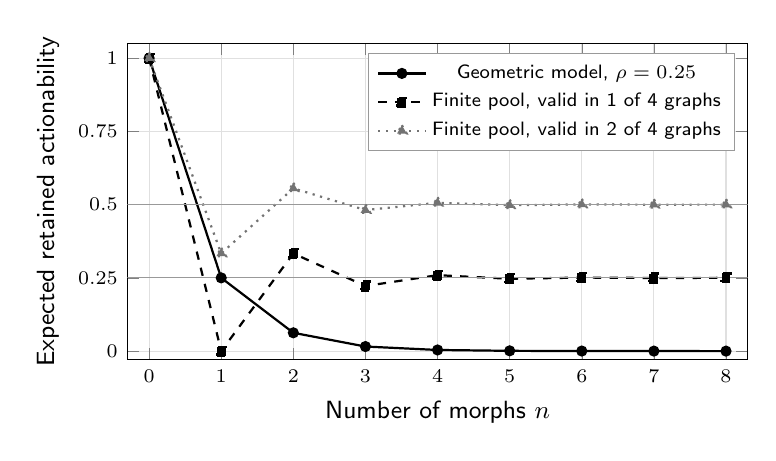
\begin{tikzpicture}
\begin{axis}[
  width=0.78\textwidth, height=5.6cm,
  xlabel={Number of morphs $n$}, ylabel={Expected retained actionability},
  xmin=-0.3, xmax=8.3, ymin=-0.03, ymax=1.05,
  xtick={0,1,...,8}, ytick={0,0.25,0.5,0.75,1},
  legend style={font=\sffamily\scriptsize, at={(0.98,0.97)}, anchor=north east, draw=black!40},
  tick label style={font=\sffamily\scriptsize}, label style={font=\sffamily\small},
  grid=major, grid style={black!12},
]
\addplot[black, thick, mark=*, mark size=1.6pt, domain=0:8, samples=9] {0.25^x};
\addlegendentry{Geometric model, $\rho=0.25$}
\addplot[black, thick, dashed, mark=square*, mark size=1.6pt, domain=0:8, samples=9] {0.25+0.75*cos(180*x)*(1/3)^x};
\addlegendentry{Finite pool, valid in 1 of 4 graphs}
\addplot[black!55, thick, dotted, mark=triangle*, mark size=2pt, domain=0:8, samples=9] {0.5+0.5*cos(180*x)*(1/3)^x};
\addlegendentry{Finite pool, valid in 2 of 4 graphs}
\addplot[black!40, thin, domain=-0.3:8.3, samples=2] {0.25};
\addplot[black!40, thin, domain=-0.3:8.3, samples=2] {0.5};
\end{axis}
\end{tikzpicture}
\caption{Retention of a structure-bound prerequisite under recurrence in a four-graph certified pool with no self-transition, compared with the geometric model. The finite pool converges to a floor equal to the stationary probability of graphs in which the prerequisite holds, not to zero.}
\label{fig:retention}
\end{figure}

These equations are models, not guarantees. They become useful only when $\rho$, $Q$, and $v_i$ are empirically estimated for a defined attacker and morph family. Correlated morph effects, persistent invariants, adaptive attackers, and multi-epoch knowledge accumulation violate the simplest models and must be measured rather than assumed away.

\subsection{Attacker completion-time model}\label{sec:completion}

A second model links morph rate and attacker speed. For an arbitrary nonnegative attacker completion-time random variable $T_A$ and effective reconnaissance-decay rate $a$, expected retained reconnaissance at attacker completion is the Laplace transform $\mathcal{L}_{T_A}(a)=E[\exp(-aT_A)]$. If $T_A$ is exponentially distributed with rate $b$ and morphs are Poisson with $a=\lambda(1-\rho)$, the expression reduces to
\begin{equation}\label{eq:completion}
E[\exp(-aT_A)]=\frac{b}{b+a}=\frac{b}{b+\lambda(1-\rho)}.
\end{equation}
Equation~\eqref{eq:completion} applies directly to epoch-bound prerequisites. For structure-bound prerequisites, Equation~\eqref{eq:markovpois} gives $E[v_i(T_A)]=R_{\infty,i}+\sum_{k\ge2}a_k\,\mathcal{L}_{T_A}\big(\lambda(1-\mu_k)\big)$, so as the morph rate grows, expected retention at attacker completion approaches the floor rather than zero. The exponential case is an illustration, not an empirical claim about attacker timing; adaptive attackers may couple $T_A$ to observed morph behavior, which is why $F_{\mathrm{evt}}$ matters.

This expression captures the strategic interaction: faster morphing helps, but so does making each morph semantically invalidate more prerequisites, and so does keeping the recurrence floor low. A high churn rate that preserves $\rho$ near one, or that cycles among a few similar graphs, can be less useful than a slower morph that sharply reduces prerequisite transfer. This is precisely why MIAM optimizes transferability and pool composition, not frequency alone.

\section{Morph Selection as a Constrained Optimization Problem}\label{sec:opt}

For each candidate $G'$, the controller evaluates prerequisite actionability, attack-path survival, absolute exposure, mutation cost, SLO risk, variant leakage, transition detectability, and state-continuity risk. It also computes a graph delta $\Delta_e(G')=\mathrm{Diff}(G_e,G')$ that records capability reassignment, dependency-edge changes, implementation changes, identity-policy changes, and affected state owners. A candidate is eligible only if the mission contract, exposure bound, and transition-safety constraints pass; the optimizer then chooses among eligible candidates rather than allowing a risk score to waive correctness.

Each objective term is mapped to $[0,1]$ before weighting: RTR, PSR, $\mathrm{Exp}$, $F_{\mathrm{obs}}$, and $F_{\mathrm{evt}}$ already lie in that range, while mutation cost $C_{\mathrm{mut}}$, SLO risk $L_{\mathrm{SLO}}$, and state risk $S_{\mathrm{state}}$ are divided by declared operator budgets and clipped, written $\hat C_{\mathrm{mut}}$, $\hat L_{\mathrm{SLO}}$, and $\hat S_{\mathrm{state}}$. The raw quantities are defined as follows, each measured or predicted for one transition from $G_e$ to $G'$:
\begin{itemize}[leftmargin=1.5em,itemsep=1pt]
\item $C_{\mathrm{mut}}$: additional compute consumed by the transition, in CPU-core-seconds summed over dark instantiation, pre-warming, state transfer, and overlap, plus control-plane and KMS operations weighted by a declared per-operation cost; budget $B_C$ per transition.
\item $L_{\mathrm{SLO}}$: the fraction of the service's SLO error budget for the current rolling window that the transition is predicted to consume, estimated from staging load tests and canary history; budget $B_L$.
\item $S_{\mathrm{state}}$: the sensitivity-weighted fraction of registered mission-domain objects that must cross the SCF under $P_{\mathrm{state}}$, plus a fixed penalty for each crossing object class that has no target-specific validator; budget $B_S$.
\end{itemize}
Each normalized term is $\hat x=\min(1,x/B_x)$ with $B_x>0$ declared before operation.
\begin{equation}\label{eq:J}
J(G')=\lambda_R\,\mathrm{RTR}+\lambda_P\,\mathrm{PSR}+\lambda_X\,\mathrm{Exp}+\lambda_C\,\hat C_{\mathrm{mut}}+\lambda_L\,\hat L_{\mathrm{SLO}}+\lambda_F\,F_{\mathrm{obs}}+\lambda_V\,F_{\mathrm{evt}}+\lambda_S\,\hat S_{\mathrm{state}}
\end{equation}
\begin{equation}\label{eq:select}
\begin{aligned}
G_{e+1}=\arg\min_{G'\in\Omega_M}\ &J(G')\\
\text{subject to}\ &G'\ \text{admissible under Eq.~\eqref{eq:admissible}},\quad \mathrm{VerifyStatePolicy}\big(P_{\mathrm{state}}(G')\big)=\mathrm{PASS},\\
&\mathrm{RTR}(K_{\le e},G')\le 1-r_{\min},\quad
\mathrm{Exp}_{X_v}(G')\le\mathrm{Exp}_{X_v}(G_{\mathrm{ref}})+\delta_X,\quad
D_{\mathrm{arch}}(G_e,G')\ge d_{\min}.
\end{aligned}
\end{equation}
Here $P_{\mathrm{state}}(G')=\mathrm{CompileStatePolicy}(\mathrm{Diff}(G_e,G'),M,\{\Sigma_c\})$ as defined in Section~\ref{sec:scf}. If no candidate satisfies the constraints, the controller keeps the current graph or restores a known-good graph rather than relaxing a constraint. If the number of feasible candidates falls below a declared minimum $m_{\min}$ for longer than a declared interval, the controller raises an alert, because a shrinking feasible set can indicate that an attacker is exhausting candidates through load, SLO pressure, or resource starvation.

Equation~\eqref{eq:select} constrains each individual transition. Two further constraints apply at the level of the selection policy and schedule rather than to a single candidate, and are checked whenever the certified pool, the selection policy, or the morph schedule changes: for epoch-bound prerequisites, the knowledge-retention half-time of Equations~\eqref{eq:t50det} or~\eqref{eq:t50pois} must not exceed a policy maximum $T_{\max}$; and for each high-weight structure-bound prerequisite $\kappa_i$, the recurrence floor $R_{\infty,i}=\pi(A_i)$ of Equation~\eqref{eq:markov}, computed from the stationary distribution of the selection policy, must not exceed a policy maximum $R_{\max}$. A pool, policy, or schedule that fails either check is rejected before any transition is attempted. The weights are not security constants. They are operator policy parameters that must be fixed or tuned against measured objectives. Operators that prefer not to scalarize may instead compute the Pareto front over the normalized terms and choose by lexicographic priority, for example exposure first, then RTR, then cost. In high-assurance environments, the candidate generator is a proposal engine only: the verification authority signs an approved transition manifest, and the orchestrator and key authority accept only a manifest whose graph digest, mission-contract version, state-transition policy, and authorization policy have been validated.

\begin{figure}[t]
\centering
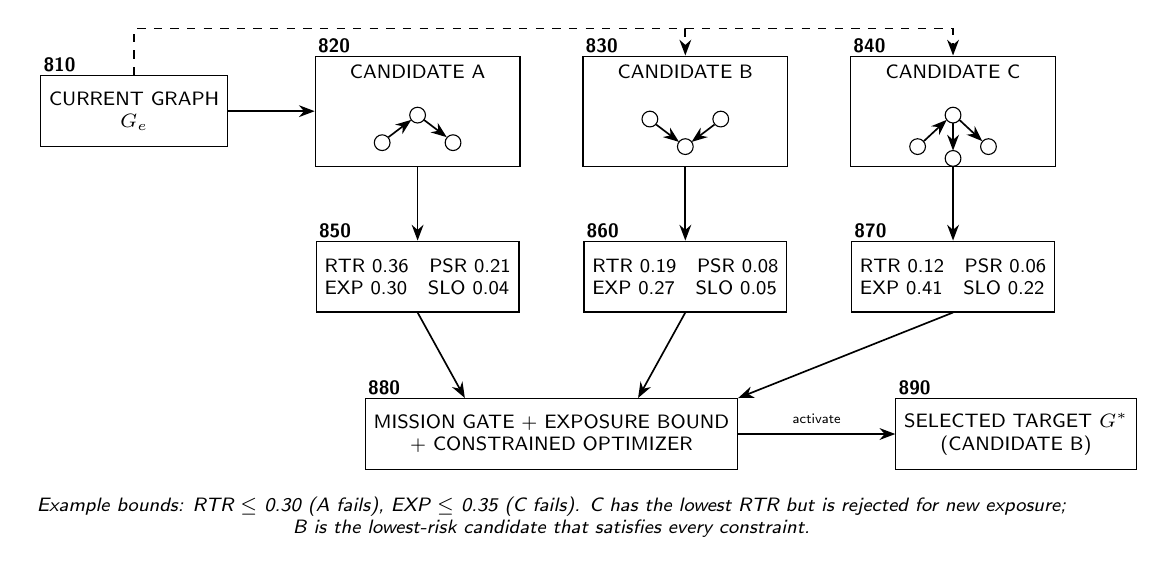
\begin{tikzpicture}[x=1cm,y=1cm]
\newcommand{\miniA}{\draw (-0.45,-0.15) circle (0.1) (0,0.2) circle (0.1) (0.45,-0.15) circle (0.1); \draw[arr] (-0.37,-0.08)--(-0.08,0.14); \draw[arr] (0.08,0.14)--(0.37,-0.08);}
\node[box, minimum width=2.3cm] (c810) at (0,2.2) {CURRENT GRAPH\\$G_e$};
\node[num] at (c810.north west) {810};
\node[box, minimum width=2.6cm, minimum height=1.4cm] (a) at (3.6,2.2) {};
\node[font=\sffamily\scriptsize, anchor=north] at (a.north) {CANDIDATE A};
\node[num] at (a.north west) {820};
\node[box, minimum width=2.6cm, minimum height=1.4cm] (b) at (7.0,2.2) {};
\node[font=\sffamily\scriptsize, anchor=north] at (b.north) {CANDIDATE B};
\node[num] at (b.north west) {830};
\node[box, minimum width=2.6cm, minimum height=1.4cm] (c) at (10.4,2.2) {};
\node[font=\sffamily\scriptsize, anchor=north] at (c.north) {CANDIDATE C};
\node[num] at (c.north west) {840};
\begin{scope}[shift={(3.6,1.95)}]\miniA\end{scope}
\begin{scope}[shift={(7.0,1.95)}]\draw (-0.45,0.15) circle (0.1) (0,-0.2) circle (0.1) (0.45,0.15) circle (0.1); \draw[arr] (-0.37,0.08)--(-0.08,-0.14); \draw[arr] (0.37,0.08)--(0.08,-0.14);\end{scope}
\begin{scope}[shift={(10.4,1.95)}]\draw (-0.45,-0.2) circle (0.1) (0,0.2) circle (0.1) (0.45,-0.2) circle (0.1) (0,-0.35) circle (0.1); \draw[arr] (-0.37,-0.13)--(-0.08,0.14); \draw[arr] (0.08,0.14)--(0.37,-0.13); \draw[arr] (0,0.1)--(0,-0.25);\end{scope}
\draw[arr] (c810.east) -- (a.west);
\draw[darr] (c810.north) |- (7.0,3.25) -- (b.north);
\draw[darr] (7.0,3.25) -| (c.north);
\node[box, minimum width=2.3cm, align=left] (s850) at (3.6,0.1) {RTR 0.36\quad PSR 0.21\\EXP 0.30\quad SLO 0.04};
\node[num] at (s850.north west) {850};
\node[box, minimum width=2.3cm, align=left] (s860) at (7.0,0.1) {RTR 0.19\quad PSR 0.08\\EXP 0.27\quad SLO 0.05};
\node[num] at (s860.north west) {860};
\node[box, minimum width=2.3cm, align=left] (s870) at (10.4,0.1) {RTR 0.12\quad PSR 0.06\\EXP 0.41\quad SLO 0.22};
\node[num] at (s870.north west) {870};
\draw[arr] (a) -- (s850); \draw[arr] (b) -- (s860); \draw[arr] (c) -- (s870);
\node[box, minimum width=4.4cm] (g880) at (5.3,-1.9) {MISSION GATE + EXPOSURE BOUND\\+ CONSTRAINED OPTIMIZER};
\node[num] at (g880.north west) {880};
\node[box, minimum width=2.9cm] (s890) at (11.2,-1.9) {SELECTED TARGET $G^*$\\(CANDIDATE B)};
\node[num] at (s890.north west) {890};
\draw[arr] (s850.south) -- (g880.north -| 4.2,0);
\draw[arr] (s860.south) -- (g880.north -| 6.4,0);
\draw[arr] (s870.south) -- (g880.north east);
\draw[arr] (g880) -- node[above, font=\sffamily\tiny]{activate} (s890);
\node[capn] at (5.3,-2.95) {Example bounds: RTR $\le$ 0.30 (A fails), EXP $\le$ 0.35 (C fails). C has the lowest RTR but is rejected for new exposure;\\B is the lowest-risk candidate that satisfies every constraint.};
\end{tikzpicture}
\caption{Candidate generation, multi-objective scoring, and constrained selection. Reference numerals are reused in Appendix A.}
\label{fig:select}
\end{figure}

\section{Why the Architecture Must Be Constrained}

Arbitrary repartitioning grows super-exponentially. The number of partitions of $n$ capability units is the Bell number $B_n$: $B_5=52$, $B_8=4{,}140$, $B_{10}=115{,}975$, $B_{15}=1{,}382{,}958{,}545$, and $B_{20}=51{,}724{,}158{,}235{,}372$. Exhaustive search over all partitions is therefore unreasonable even before dependency edges, implementation variants, placement, identity, and policy attributes are considered.

The production design uses a certified architecture grammar rather than the full Bell space. If $q$ independent variation points expose at most $b_j$ legal alternatives, the unpruned candidate bound is $N_\Gamma\le\prod_{j=1}^{q}b_j$; dependency, policy, residency, state-ownership, exposure, and mission constraints prune this set before scoring. An exhaustive bounded selector therefore scales with the number of grammar candidates actually emitted, not $B_n$, while CP-SAT/SMT, branch-and-bound, or graph search can prune earlier. The implementation goal is not maximum morph diversity. It is the best verified transition available within operational cost and a bounded decision deadline. Section~\ref{sec:retention} adds a countervailing requirement: the certified pool must still be large and diverse enough that the recurrence floor for high-weight structure-bound prerequisites stays below the operator's tolerance.

\section{MIAM System Architecture}

The MIAM system (100) comprises a control and decision plane and a runtime and transition plane. The control plane contains the Mission Contract Registry (120), Observability Graph Builder (130), attacker-knowledge model (140), candidate graph generator (150), prerequisite-actionability, exposure, and fingerprint scorer (160), verification authority (170), epoch orchestrator (180), and identity/key authority (190). The runtime and transition plane contains the stable service interface (110), the State Continuity Firewall (200), the source and target runtime graphs (210, 220), and the evidence ledger (230), which the control plane writes and auditors read. The control plane should be smaller, more static, separately authenticated, and more strongly isolated than the workloads it controls because compromise of the mutation authority would invert the defensive advantage.

A concrete trust split is required. The candidate generator has no activation privilege; the verification authority signs an immutable transition manifest; the orchestrator activates only signed manifests; and the KMS/HSM releases target-epoch material only for an authorized manifest digest and attested orchestrator identity. Telemetry used for graph and prerequisite estimation should be cross-checked across independent sources and carry provenance. Morph triggers are rate-limited and use hysteresis so an attacker cannot cheaply force repeated transitions. On control-plane uncertainty, the fail-safe action is to retain or restore a known-good graph rather than explore a new one.

\begin{figure}[t]
\centering
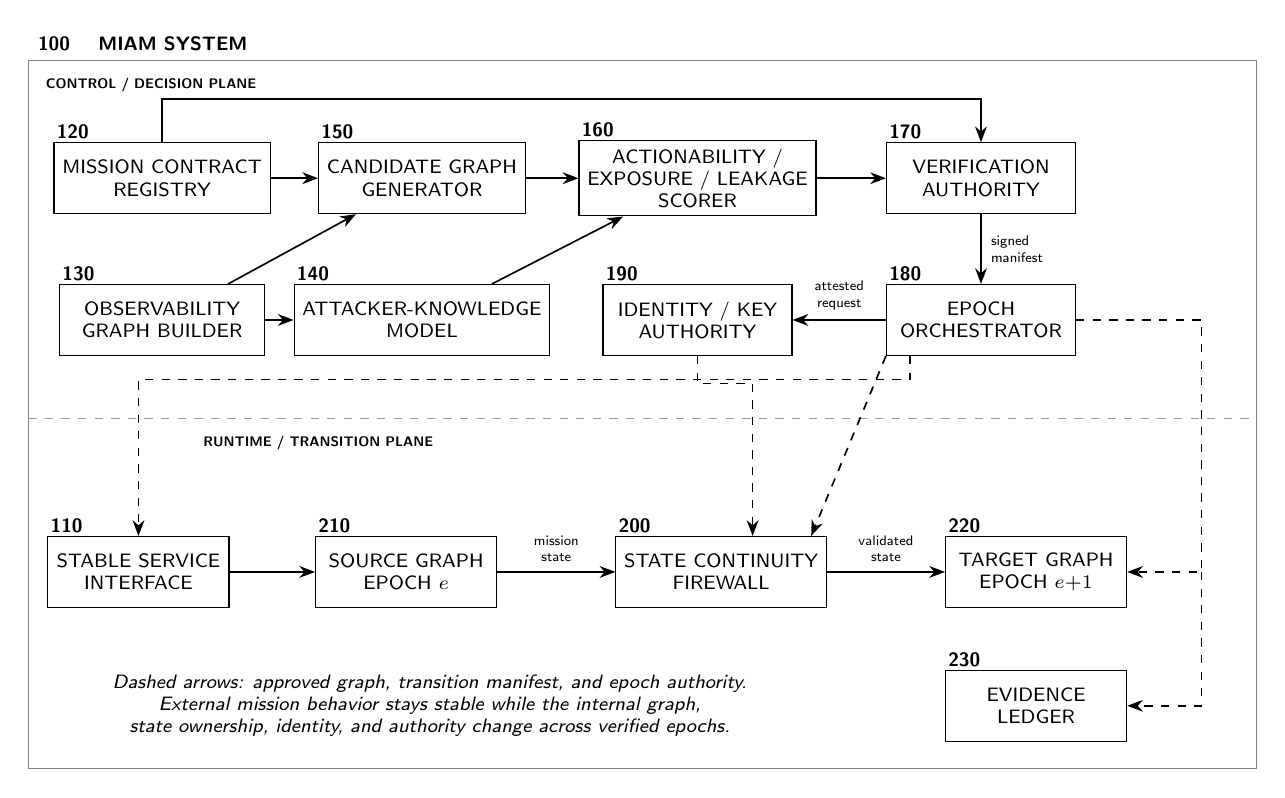
\begin{tikzpicture}[x=1cm,y=1cm]
\draw[black!50] (-0.5,5.9) rectangle (15.1,-3.1);
\node[font=\sffamily\scriptsize\bfseries, anchor=south west] at (-0.5,5.9) {100 \quad MIAM SYSTEM};
\node[font=\sffamily\tiny\bfseries, anchor=north west] at (-0.4,5.8) {CONTROL / DECISION PLANE};
\node[box, minimum width=2.6cm] (n120) at (1.2,4.4) {MISSION CONTRACT\\REGISTRY};
\node[num] at (n120.north west) {120};
\node[box, minimum width=2.6cm] (n130) at (1.2,2.6) {OBSERVABILITY\\GRAPH BUILDER};
\node[num] at (n130.north west) {130};
\node[box, minimum width=2.6cm] (n140) at (4.5,2.6) {ATTACKER-KNOWLEDGE\\MODEL};
\node[num] at (n140.north west) {140};
\node[box, minimum width=2.6cm] (n150) at (4.5,4.4) {CANDIDATE GRAPH\\GENERATOR};
\node[num] at (n150.north west) {150};
\node[box, minimum width=3.0cm] (n160) at (8.0,4.4) {ACTIONABILITY /\\EXPOSURE / LEAKAGE\\SCORER};
\node[num] at (n160.north west) {160};
\node[box, minimum width=2.4cm] (n170) at (11.6,4.4) {VERIFICATION\\AUTHORITY};
\node[num] at (n170.north west) {170};
\node[box, minimum width=2.4cm] (n180) at (11.6,2.6) {EPOCH\\ORCHESTRATOR};
\node[num] at (n180.north west) {180};
\node[box, minimum width=2.4cm] (n190) at (8.0,2.6) {IDENTITY / KEY\\AUTHORITY};
\node[num] at (n190.north west) {190};
\draw[arr] (n120) -- (n150);
\draw[arr] (n130) -- (n150);
\draw[arr] (n130) -- (n140);
\draw[arr] (n140) -- (n160);
\draw[arr] (n150) -- (n160);
\draw[arr] (n160) -- (n170);
\draw[arr] (n120.north) -- ++(0,0.55) -| (n170.north);
\draw[arr] (n170) -- node[right, font=\sffamily\tiny, align=left]{signed\\manifest} (n180);
\draw[arr] (n180) -- node[above, font=\sffamily\tiny, align=center]{attested\\request} (n190);
\draw[black!40, dashed] (-0.5,1.35) -- (15.1,1.35);
\node[font=\sffamily\tiny\bfseries, anchor=north west] at (1.6,1.25) {RUNTIME / TRANSITION PLANE};
\node[box, minimum width=2.3cm] (n110) at (0.9,-0.6) {STABLE SERVICE\\INTERFACE};
\node[num] at (n110.north west) {110};
\node[box, minimum width=2.3cm] (n210) at (4.3,-0.6) {SOURCE GRAPH\\EPOCH $e$};
\node[num] at (n210.north west) {210};
\node[box, minimum width=2.3cm] (n200) at (8.3,-0.6) {STATE CONTINUITY\\FIREWALL};
\node[num] at (n200.north west) {200};
\node[box, minimum width=2.3cm] (n220) at (12.3,-0.6) {TARGET GRAPH\\EPOCH $e{+}1$};
\node[num] at (n220.north west) {220};
\node[box, minimum width=2.3cm] (n230) at (12.3,-2.3) {EVIDENCE\\LEDGER};
\node[num] at (n230.north west) {230};
\draw[arr] (n110) -- (n210);
\draw[arr] (n210) -- node[above, font=\sffamily\tiny, align=center]{mission\\state} (n200);
\draw[arr] (n200) -- node[above, font=\sffamily\tiny, align=center]{validated\\state} (n220);
\draw[darr] (n180.east) -- (14.4,2.6) |- (n220.east);
\draw[darr] (n180.south west) -- ([xshift=-2mm]n200.north east);
\draw[darr] (14.4,-0.6) |- (n230.east);
\draw[darr] (n180.south) ++(-0.9,0) -- ++(0,-0.3) -| (n110.north);
\draw[darr] (n190.south) -- ++(0,-0.35) -| ([xshift=4mm]n200.north);
\node[capn] at (4.6,-2.3) {Dashed arrows: approved graph, transition manifest, and epoch authority.\\External mission behavior stays stable while the internal graph,\\state ownership, identity, and authority change across verified epochs.};
\end{tikzpicture}
\caption{Reference architecture for mission-invariant service-graph morphing.}
\label{fig:arch}
\end{figure}

The lifecycle is observe, generate, score, verify, prepare, transfer and rehydrate, cut over, revoke/retire, and learn (Figure~\ref{fig:lifecycle}). Morph triggers may be periodic, risk-adaptive, operator initiated, incident driven, or chosen by an optimization policy. Purely deterministic schedules are easier to operate but more predictable and easier to detect; purely random schedules can waste resources. The preferred design combines bounded randomization with risk and mission constraints.

\begin{figure}[t]
\centering
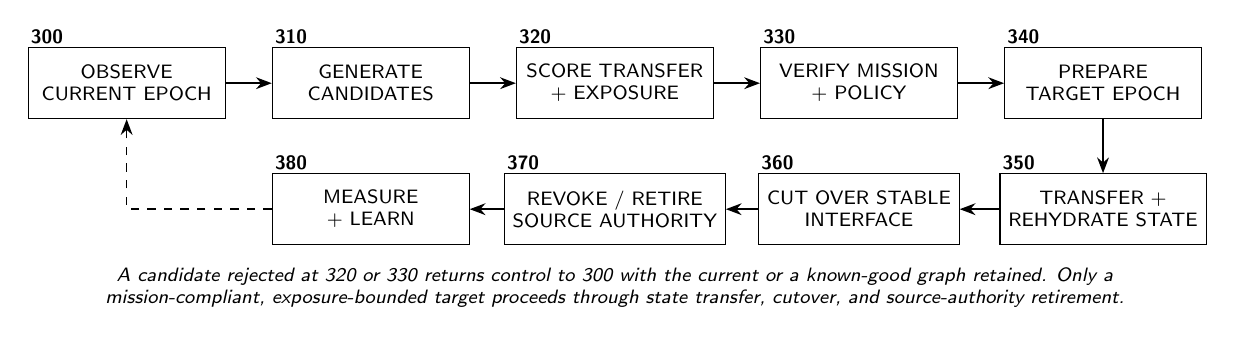
\begin{tikzpicture}[x=1cm,y=1cm]
\foreach \n/\t/\x in {300/{OBSERVE\\CURRENT EPOCH}/0, 310/{GENERATE\\CANDIDATES}/3.1, 320/{SCORE TRANSFER\\+ EXPOSURE}/6.2, 330/{VERIFY MISSION\\+ POLICY}/9.3, 340/{PREPARE\\TARGET EPOCH}/12.4} {
  \node[box, minimum width=2.5cm] (l\n) at (\x,1.6) {\t};
  \node[num] at (l\n.north west) {\n};
}
\foreach \n/\t/\x in {380/{MEASURE\\+ LEARN}/3.1, 370/{REVOKE / RETIRE\\SOURCE AUTHORITY}/6.2, 360/{CUT OVER STABLE\\INTERFACE}/9.3, 350/{TRANSFER +\\REHYDRATE STATE}/12.4} {
  \node[box, minimum width=2.5cm] (l\n) at (\x,0) {\t};
  \node[num] at (l\n.north west) {\n};
}
\draw[arr] (l300)--(l310); \draw[arr] (l310)--(l320); \draw[arr] (l320)--(l330); \draw[arr] (l330)--(l340);
\draw[arr] (l340)--(l350); \draw[arr] (l350)--(l360); \draw[arr] (l360)--(l370); \draw[arr] (l370)--(l380);
\draw[darr] (l380.west) -| (l300.south);
\node[capn] at (6.2,-1.0) {A candidate rejected at 320 or 330 returns control to 300 with the current or a known-good graph retained. Only a\\mission-compliant, exposure-bounded target proceeds through state transfer, cutover, and source-authority retirement.};
\end{tikzpicture}
\caption{Epoch transition lifecycle with closed-loop evidence feedback.}
\label{fig:lifecycle}
\end{figure}

\section{Service-Graph Morphing Mechanisms}

Each morph changes one or more attack-relevant internal properties while preserving the mission contract. Service fusion can remove a network-visible trust edge but raises privilege concentration; service fission can create a new mediation boundary but may add edges; implementation substitution can change a vulnerability family; policy-mediator insertion can force a new authorization path; dependency rerouting can alter traversal; and placement or substrate changes can reduce reuse of host-specific knowledge. The system records the source-to-target graph delta and prefers transitions whose measured or predicted prerequisite actionability is materially lower without raising absolute exposure, not transitions that are merely structurally different. Figure~\ref{fig:partition} shows a service-boundary morph.

\begin{figure}[t]
\centering
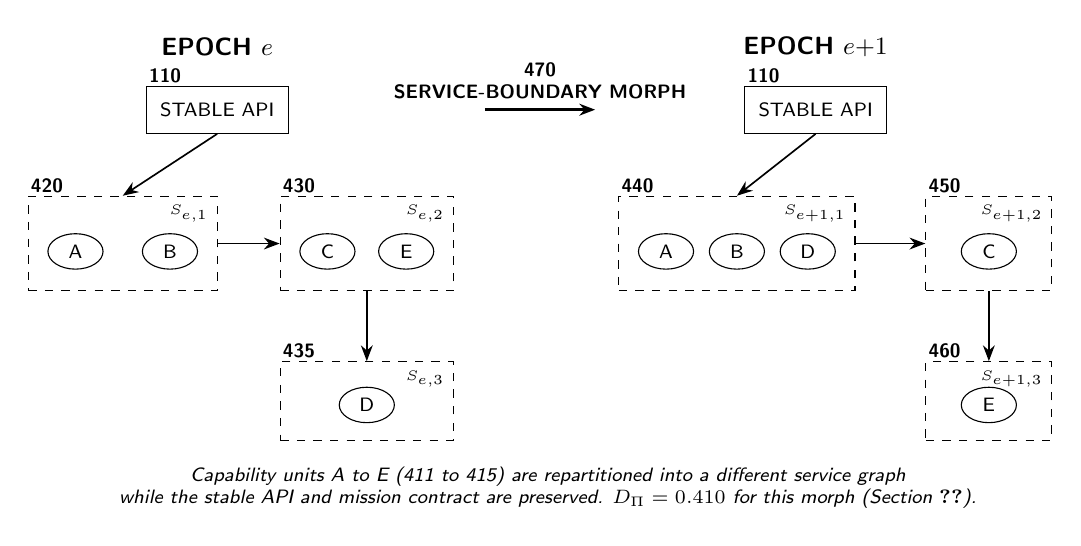
\begin{tikzpicture}[x=1cm,y=1cm]
\newcommand{\svc}[5]{\node[draw, dashed, minimum width=#3cm, minimum height=#4cm] (#1) at #2 {}; \node[font=\sffamily\tiny\itshape, anchor=north east] at (#1.north east) {#5};}
\node[font=\sffamily\small\bfseries] at (2.4,4.1) {EPOCH $e$};
\node[font=\sffamily\small\bfseries] at (10.0,4.1) {EPOCH $e{+}1$};
\node[box, minimum width=1.8cm, minimum height=6mm] (api1) at (2.4,3.3) {STABLE API};
\node[num] at (api1.north west) {110};
\node[box, minimum width=1.8cm, minimum height=6mm] (api2) at (10.0,3.3) {STABLE API};
\node[num] at (api2.north west) {110};
\svc{p420}{(1.2,1.6)}{2.4}{1.2}{$S_{e,1}$}
\node[num] at (p420.north west) {420};
\svc{p430}{(4.3,1.6)}{2.2}{1.2}{$S_{e,2}$}
\node[num] at (p430.north west) {430};
\svc{p435}{(4.3,-0.4)}{2.2}{1.0}{$S_{e,3}$}
\node[num] at (p435.north west) {435};
\node[cu] at (0.6,1.5) {A}; \node[cu] at (1.8,1.5) {B};
\node[cu] at (3.8,1.5) {C}; \node[cu] at (4.8,1.5) {E};
\node[cu] at (4.3,-0.45) {D};
\draw[arr] (api1.south) -- (p420.north);
\draw[arr] (p420.east) -- (p430.west);
\draw[arr] (p430.south) -- (p435.north);
\svc{p440}{(9.0,1.6)}{3.0}{1.2}{$S_{e+1,1}$}
\node[num] at (p440.north west) {440};
\svc{p450}{(12.2,1.6)}{1.6}{1.2}{$S_{e+1,2}$}
\node[num] at (p450.north west) {450};
\svc{p460}{(12.2,-0.4)}{1.6}{1.0}{$S_{e+1,3}$}
\node[num] at (p460.north west) {460};
\node[cu] at (8.1,1.5) {A}; \node[cu] at (9.0,1.5) {B}; \node[cu] at (9.9,1.5) {D};
\node[cu] at (12.2,1.5) {C};
\node[cu] at (12.2,-0.45) {E};
\draw[arr] (api2.south) -- (p440.north);
\draw[arr] (p440.east) -- (p450.west);
\draw[arr] (p450.south) -- (p460.north);
\draw[arr, very thick] (5.8,3.3) -- node[above, font=\sffamily\scriptsize\bfseries, align=center]{470\\SERVICE-BOUNDARY MORPH} (7.2,3.3);
\node[capn] at (6.6,-1.5) {Capability units A to E (411 to 415) are repartitioned into a different service graph\\while the stable API and mission contract are preserved. $D_\Pi=0.410$ for this morph (Section~\ref{sec:checks}).};
\end{tikzpicture}
\caption{Example change in capability-to-service partition while the stable service interface and mission capabilities remain unchanged.}
\label{fig:partition}
\end{figure}

Runtime microservice decomposition and service reconstruction are themselves known in the patent literature, including runtime decomposition for distributed execution and recent dependency-graph-driven reconstruction techniques \cite{cn121116381,ep4046020,cn120743522}, and runtime rotation among implementation variants has been demonstrated on Kubernetes \cite{gonzalez2023}. Therefore, MIAM's claim-oriented distinction is the security selection loop and epoch lifecycle, not the general ability to split, merge, or diversify services.

\section{State Continuity Firewall}\label{sec:scf}

State continuity is where a moving architecture can accidentally preserve an attacker foothold. A conventional stateful migration can carry process memory, compromised caches, runtime tokens, injected libraries, or contaminated temporary artifacts into the target. MIAM therefore treats state movement as a derived transition policy rather than a generic copy operation. Mission-domain state is defined as typed state explicitly required by the mission contract or a registered capability-state contract to continue externally required behavior; being syntactically valid business data is not sufficient.

For each capability $c$, a capability-state contract $\Sigma_c=(T_c,V_c,R_c,X_c)$ declares transferable mission-domain object types $T_c$, required validators $V_c$, target reconstruction rules $R_c$, and prohibited runtime/security classes $X_c$. Given $\Delta_e=\mathrm{Diff}(G_e,G_{e+1})$, the transition planner compiles $P_{\mathrm{state}}=\mathrm{CompileStatePolicy}(\Delta_e,M,\{\Sigma_c\})$. State classification is therefore tied to the actual capability ownership and boundary changes of the selected morph rather than to a global label such as ``semantic.''

A state object may cross the SCF only if its type is allowed for the mapped target capability; its schema, provenance, integrity, authorization, freshness, and replay sequence validate; all mission/business invariants for that object hold; content-safety checks relevant to the target parser or deserializer pass; and the object is not a prohibited executable, credential, source-epoch token, process snapshot, hook, or local runtime secret. Durable mission records may pass after these gates. User-continuity state is reauthorized or rebound. Caches and derived indexes are rebuilt. Locks are reacquired under new fencing epochs. Source cryptographic material never crosses.

This stronger rule addresses malicious-but-valid business state. A payload can satisfy a schema yet still exploit a target parser or encode a dangerous workflow value. The SCF therefore applies target-specific semantic invariants, canonicalization, bounded parsing, content validation, and where applicable taint or provenance policy before rehydration. Failure is fail-closed: the object is quarantined and the target epoch remains uncommitted, or the transition is aborted if the object is mission-required. No partial interface cutover occurs merely to preserve availability.

\begin{figure}[t]
\centering
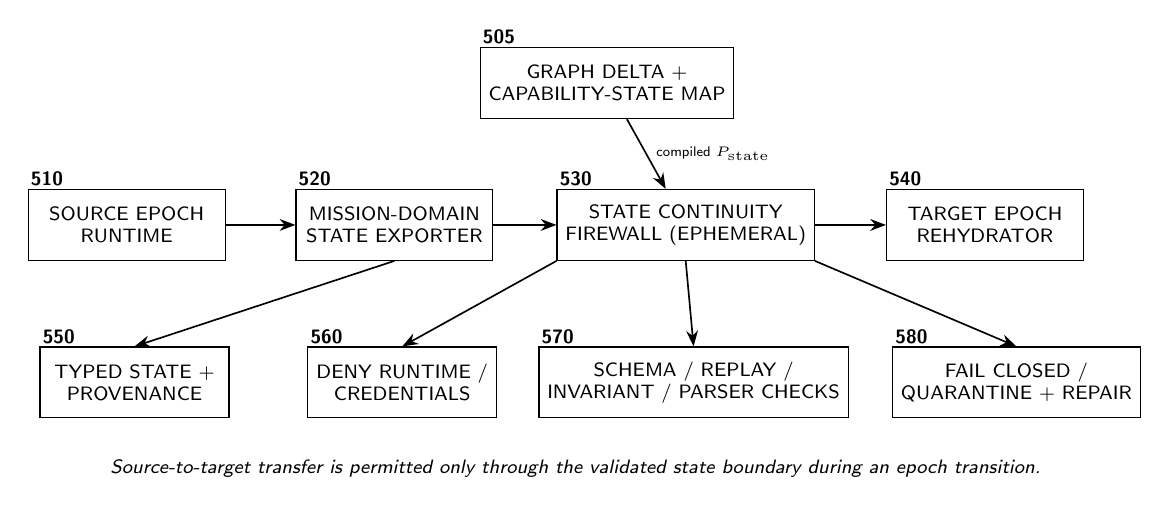
\begin{tikzpicture}[x=1cm,y=1cm]
\node[box, minimum width=3.2cm] (s505) at (7.0,2.4) {GRAPH DELTA +\\CAPABILITY-STATE MAP};
\node[num] at (s505.north west) {505};
\node[box, minimum width=2.5cm] (s510) at (0.9,0.6) {SOURCE EPOCH\\RUNTIME};
\node[num] at (s510.north west) {510};
\node[box, minimum width=2.5cm] (s520) at (4.3,0.6) {MISSION-DOMAIN\\STATE EXPORTER};
\node[num] at (s520.north west) {520};
\node[box, minimum width=2.9cm] (s530) at (8.0,0.6) {STATE CONTINUITY\\FIREWALL (EPHEMERAL)};
\node[num] at (s530.north west) {530};
\node[box, minimum width=2.5cm] (s540) at (11.8,0.6) {TARGET EPOCH\\REHYDRATOR};
\node[num] at (s540.north west) {540};
\draw[arr] (s510)--(s520); \draw[arr] (s520)--(s530); \draw[arr] (s530)--(s540);
\draw[arr] (s505) -- node[right, font=\sffamily\tiny]{compiled $P_{\mathrm{state}}$} (s530);
\node[box, minimum width=2.4cm] (s550) at (1.0,-1.4) {TYPED STATE +\\PROVENANCE};
\node[num] at (s550.north west) {550};
\node[box, minimum width=2.4cm] (s560) at (4.4,-1.4) {DENY RUNTIME /\\CREDENTIALS};
\node[num] at (s560.north west) {560};
\node[box, minimum width=2.9cm] (s570) at (8.1,-1.4) {SCHEMA / REPLAY /\\INVARIANT / PARSER CHECKS};
\node[num] at (s570.north west) {570};
\node[box, minimum width=2.7cm] (s580) at (12.2,-1.4) {FAIL CLOSED /\\QUARANTINE + REPAIR};
\node[num] at (s580.north west) {580};
\draw[arr] (s520.south) -- (s550.north);
\draw[arr] (s530.south west) -- (s560.north);
\draw[arr] (s530.south) -- (s570.north);
\draw[arr] (s530.south east) -- (s580.north);
\node[capn] at (6.6,-2.5) {Source-to-target transfer is permitted only through the validated state boundary during an epoch transition.};
\end{tikzpicture}
\caption{State Continuity Firewall: graph-delta-derived transfer policy, mission-domain state validation, runtime-state denial, and target reconstruction.}
\label{fig:scf}
\end{figure}

The transfer manifest includes source and target epochs, graph digests, the graph delta, source-to-target capability mapping, object type, schema version, object identifier, monotonic sequence or nonce, provenance, authorization decision, validation policy version, and integrity/authentication evidence. During the overlap window, direct source-to-target workload calls are denied; the SCF transfer channel is the only authorized cross-epoch data path. A raw VM or container snapshot is never equivalent to mission-domain state.

\paragraph{Hardening the SCF.} The SCF parses attacker-influenceable data exported from a possibly compromised source while holding transfer keys for both epochs, which makes it the highest-value component in the transition path. It should be instantiated fresh for each transition from a signed image, hold no persistent state beyond the transition, use memory-safe and bounded parsers, run with no network path other than the source export and target import channels, and be destroyed after the transition commits or aborts. A trusted execution boundary is an optional additional layer.

\paragraph{Pinning detection and containment.} Fail-closed abort on mission-required objects creates a denial-of-morph risk: an attacker who plants one malformed but mission-required record could block every future transition and pin the system to a graph the attacker has already mapped. The SCF therefore routes a failed mission-required object to a quarantine-and-repair path (operator review, reconstruction from an authoritative system of record, or reissue by the owning business process) with a bounded retry budget. Repeated aborts attributable to the same object class or origin are raised as a security incident, and the orchestrator records the pinned duration in the evidence ledger so that extended pinning is visible rather than silent. When the pinned duration exceeds a declared threshold, the orchestrator applies containment to the pinned graph rather than waiting for a successful morph: it rotates epoch keys and workload identities in place, which invalidates epoch-bound prerequisites without any state crossing the SCF, and it isolates the capability that owns the failing object class behind a policy-enforcement point. These controls provide detection and containment, not a liveness guarantee. An attacker who can continuously inject distinct mission-required failures, or make the authoritative repair source unavailable, can still prevent service-graph morphing indefinitely. Forward progress for structure-bound prerequisites depends on the stated assumption that at least one authoritative reconstruction source for each mission-required object class remains available and uncompromised.

\paragraph{Overlap window and source writes.} A compromised source may remain active during overlap and attempt to race writes, destructive actions, or tampering with the export. MIAM therefore revokes source write authority at the transition fence: after the fence, the source has read-only access to the fenced snapshot that the exporter reads, and all mission writes are either rejected or queued for the target owner. The export is taken only from the fenced snapshot, and the snapshot digest is recorded in the transition manifest. The overlap window has a declared maximum duration $T_{\mathrm{ov}}$; if cutover has not completed by then, the orchestrator aborts and restores rather than extending the overlap. Destructive actions a compromised source completes before the fence are outside what a transition can undo and are handled by conventional backup and incident response.

\section{Cryptographic Epoch Isolation}

\subsection{Key hierarchy and graph binding}

Cryptography should support the morph rather than become the novelty by itself. For each epoch $e$, the key authority generates an independent fresh 256-bit epoch master key $K_e$ inside a CSPRNG-backed KMS or HSM. The target key is not derived from the source key. This is important: compromise of $K_e$ should not provide the derivation chain for $K_{e+1}$. NIST key-management guidance emphasizes lifecycle controls for cryptographic material; MIAM adds epoch scoping to that operational lifecycle \cite{nist80057,nist800133}.
\begin{equation}
K_e\xleftarrow{\$}\{0,1\}^{256}\quad\text{independently for each epoch } e
\end{equation}
The controller canonicalizes the approved graph, mission-contract version, and policy version and hashes them to produce a graph context $h_e$. Canonicalization must be deterministic and unambiguous: the graph is serialized with a canonical encoding such as RFC 8785 JSON canonicalization \cite{rfc8785} or the core deterministic encoding of CBOR defined in RFC 8949 \cite{rfc8949}. Every multi-field input below is written $\langle\cdot\rangle$ and denotes a tuple encoding in which each field carries a fixed-width type tag and a fixed-width 32-bit big-endian length followed by its bytes, with the number of fields fixed per context label. Raw concatenation is never used, so no two distinct tuples share an encoding. SHA-256 is an example secure hash standardized by NIST; the architecture should remain algorithm-agile \cite{fips1804}.
\begin{equation}
h_e=\mathrm{SHA\text{-}256}\big(\langle\mathrm{Canon}(G_e),\,M_{\mathrm{version}},\,\mathrm{Policy}_{\mathrm{version}}\rangle\big)
\end{equation}
Because $K_e$ is already a uniformly random key, no extraction step is needed; a single expansion step suffices. Scoped keys are derived with a PRF-based key derivation function keyed by $K_e$, for example HKDF-Expand with SHA-256 \cite{rfc5869} or, in FIPS-validated deployments, a KDF in counter or feedback mode from NIST SP 800-108 keyed by $K_e$ as a key-derivation key \cite{nist800108,nist800133}. The SP 800-56C two-step procedure is specified for shared secrets produced by key establishment and is not the relevant path here \cite{nist80056c}.
\begin{equation}\label{eq:kdf}
K_{e,s,p,j}=\mathrm{KDF}\big(K_e,\ \langle\texttt{"MIAM-v1"},\,\mathrm{epoch\_uuid}_e,\,\mathrm{service}_s,\,\mathrm{purpose}_p,\,\mathrm{inst}_j,\,h_e\rangle,\ 256\big)
\end{equation}
For purposes other than state transfer, $\mathrm{inst}_j$ is a fixed empty field. For the state-transfer purpose, $\mathrm{inst}_j$ is a 128-bit identifier generated by the KMS/HSM from its CSPRNG when an SCF instance is created, bound into the signed transition manifest, and recorded in the evidence ledger. The KMS/HSM refuses to perform a transfer-purpose derivation for any $\mathrm{inst}_j$ it has already served. A restarted or replicated SCF therefore always receives a new identifier and a new key, so an instance-local nonce counter that restarts at zero never repeats a (key, nonce) pair.
The derivation context is public. Security comes from the independent secret $K_e$ and the KMS/HSM authorization boundary, not from hiding the graph digest or epoch identifier. Derivation should occur inside the KMS/HSM boundary so that $K_e$ is never exported; where a KMS cannot perform the chosen KDF internally, the design must state where $K_e$ is exposed and treat that component as part of the key authority's trust boundary.

Under an ideal independent-key model, $I(K_e;K_{e+1})=0$. In implementation terms this should be called cross-epoch key independence or epoch key isolation, not session forward secrecy. Computational separation depends on the entropy source, KMS/HSM isolation, authorization policy, and independent key-generation events. Deleting a live epoch key does not imply every escrow, backup, forensic, or recovery copy has vanished; those domains require separate governance.
\begin{equation}
\text{Ideal cross-epoch independence: } I(K_e;K_{e+1})=0
\end{equation}

\subsection{AEAD-protected mission-domain transfer}

State-transfer objects should use authenticated encryption with associated data (AEAD). AES-GCM is one standardized option; NIST SP 800-38D requires IV uniqueness within a key context and protects both ciphertext and associated-data authenticity \cite{nist80038d}. NIST is revising SP 800-38D, including removing authentication tags shorter than 96 bits and clarifying IV-construction guidance \cite{nist80038dr1}; MIAM profiles use 128-bit tags. The preferred profile allocates a dedicated transfer key per epoch, service, purpose, and SCF instance, with a 96-bit nonce from an instance-local monotonic counter. Because each SCF instance derives its transfer key with a never-reused $\mathrm{inst}_j$ in Equation~\eqref{eq:kdf}, counter state never needs to survive a crash or be shared across replicas; a restarted instance receives a new identifier and key rather than resuming a counter. Deployments that cannot guarantee per-instance keys should use a nonce-misuse-resistant AEAD such as AES-GCM-SIV \cite{rfc8452}.
\begin{align}
\mathrm{nonce}&=\mathrm{Encode}_{96}(\mathrm{instance\_local\_counter})\\
(C,T)&=\mathrm{AEAD\_Enc}(K_{\mathrm{state}},\,\mathrm{nonce},\,P,\,\mathrm{AAD})\\
\mathrm{AAD}&=\langle\mathrm{key\_id},\,\mathrm{src\_epoch},\,\mathrm{dst\_epoch},\,\mathrm{direction},\,\mathrm{manifest\_digest},\notag\\
&\qquad\ \mathrm{service\_id},\,\mathrm{schema\_id},\,\mathrm{object\_id},\,\mathrm{sequence}\rangle
\end{align}
The manifest digest commits to both the source and target graph digests, the graph delta, and $\mathrm{inst}_j$, so each object is bound to one specific transition rather than to one graph. The SCF selects each decryption key from the signed transition manifest, never from a field in the object itself. AES-GCM is not key-committing, and a receiver that chooses among candidate keys based on attacker-controlled input can be exposed to partitioning-oracle attacks \cite{len2021}; binding the key identifier in the AAD and fixing the key by manifest removes that choice. The SCF decrypts and authenticates under a source-epoch transfer key, rejects any object whose source epoch, sequence, graph context, or authorization is not currently permitted, applies the compiled state policy and target-specific validators, and re-encrypts accepted objects under an independently derived target-epoch transfer key. Validation failure causes quarantine, repair, or transition abort according to Section~\ref{sec:scf}. Durable business data normally remains under a separate long-lived data-encryption/key-encryption hierarchy so retirement of transient epoch keys cannot destroy required records.

\subsection{Workload identity, mTLS, and crypto agility}

Workload identities should be short-lived and epoch-aware. SPIFFE provides standardized workload identities and short-lived X.509 SVIDs that can establish mutual TLS between workloads \cite{spiffe}. If all epochs share one trust domain and one issuing CA, epoch isolation rests entirely on the authorization gate. SPIFFE itself defines workload identity and SVID delivery; it does not define epochs. The following rules are therefore a MIAM identity profile layered on SPIFFE, not SPIFFE-provided semantics. The epoch is encoded in the workload identity (for example, as a path segment of the SPIFFE ID), and, where the identity system supports it, each epoch's SVIDs are issued from a distinct intermediate CA under the same trust-domain root. During overlap, target-epoch services accept only target-epoch identities for target-epoch service boundaries, and the SCF channel is the only path that accepts both. At retirement, the source intermediate is removed from the published trust bundle and its signing key is destroyed. A rollback never reactivates a retired epoch: it instantiates the known-good graph as a new epoch with a new intermediate. If a trust-bundle update fails to propagate, affected target services continue to reject source identities, because the authorization gate below does not depend on bundle state. MIAM does not rely on certificate revocation alone for immediate epoch separation: an authorization gate checks the signed active/overlap epoch manifest and rejects a source-epoch principal at target-epoch service boundaries even if its certificate has not yet expired, and the gate fails closed if the manifest cannot be verified. Long-lived connections are drained, sent an application/protocol reconnect signal where available, or pinned to the source graph until an explicit deadline; they are not silently migrated as authenticated target-epoch sessions. Direct source-to-target service calls remain denied except through the SCF transfer channel.

Algorithm identifiers belong in a versioned cryptographic policy rather than in the core control logic. NIST's 2026 crypto-agility guidance emphasizes the ability to replace algorithms while maintaining ongoing operations \cite{nistcswp39}. A future enterprise profile may support NIST-standardized ML-KEM for quantum-resistant key establishment and ML-DSA for signatures, but post-quantum algorithms are implementation options, not the central concept \cite{fips203,fips204}.

\begin{figure}[t]
\centering
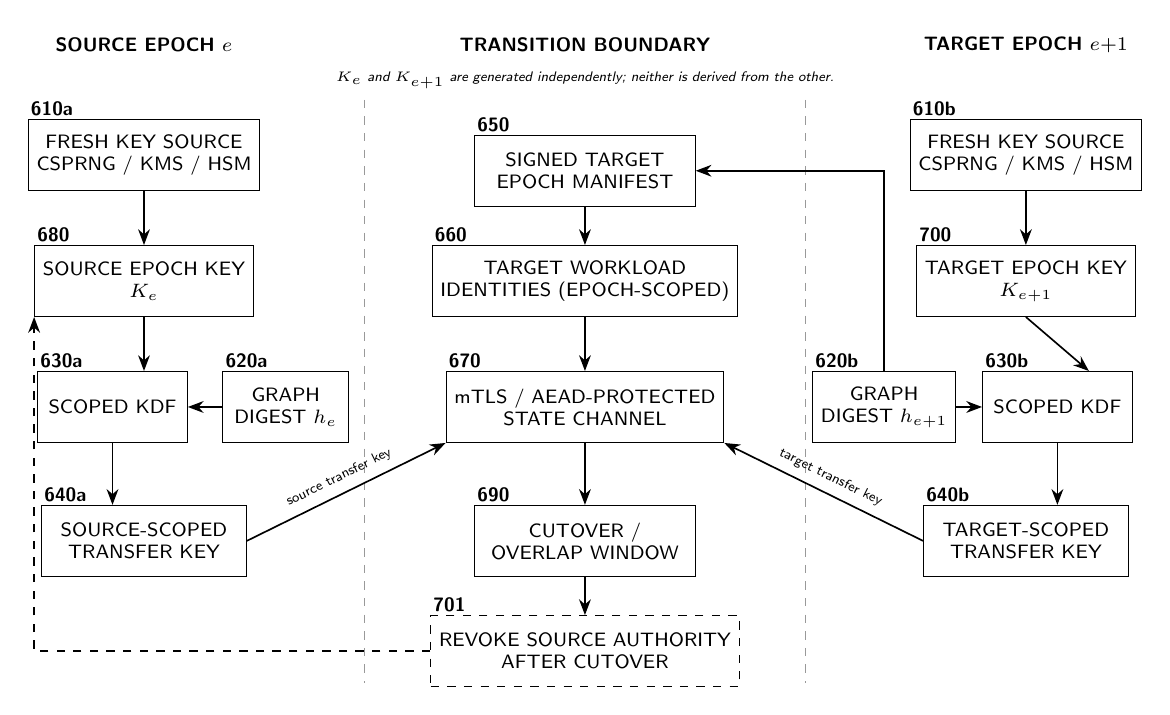
\begin{tikzpicture}[x=1cm,y=1cm]
\node[font=\sffamily\scriptsize\bfseries] at (1.4,6.9) {SOURCE EPOCH $e$};
\node[font=\sffamily\scriptsize\bfseries] at (7.0,6.9) {TRANSITION BOUNDARY};
\node[font=\sffamily\scriptsize\bfseries] at (12.6,6.9) {TARGET EPOCH $e{+}1$};
\draw[black!40, dashed] (4.2,6.2) -- (4.2,-1.2);
\draw[black!40, dashed] (9.8,6.2) -- (9.8,-1.2);
\node[font=\sffamily\tiny\itshape, fill=white] at (7.0,6.45) {$K_e$ and $K_{e+1}$ are generated independently; neither is derived from the other.};
% source
\node[box, minimum width=2.6cm] (k610a) at (1.4,5.5) {FRESH KEY SOURCE\\CSPRNG / KMS / HSM};
\node[num] at (k610a.north west) {610a};
\node[box, minimum width=2.6cm] (k680) at (1.4,3.9) {SOURCE EPOCH KEY\\$K_e$};
\node[num] at (k680.north west) {680};
\node[box, minimum width=1.6cm] (k620a) at (3.2,2.3) {GRAPH\\DIGEST $h_e$};
\node[num] at (k620a.north west) {620a};
\node[box, minimum width=1.9cm] (k630a) at (1.0,2.3) {SCOPED KDF};
\node[num] at (k630a.north west) {630a};
\node[box, minimum width=2.6cm] (k640a) at (1.4,0.6) {SOURCE-SCOPED\\TRANSFER KEY};
\node[num] at (k640a.north west) {640a};
\draw[arr] (k610a)--(k680); \draw[arr] (k680.south) -- (k630a.north -| k680.south); \draw[arr] (k620a)--(k630a); \draw[arr] (k630a.south) -- (k640a.north -| k630a.south);
% target
\node[box, minimum width=2.6cm] (k610b) at (12.6,5.5) {FRESH KEY SOURCE\\CSPRNG / KMS / HSM};
\node[num] at (k610b.north west) {610b};
\node[box, minimum width=2.6cm] (k700) at (12.6,3.9) {TARGET EPOCH KEY\\$K_{e+1}$};
\node[num] at (k700.north west) {700};
\node[box, minimum width=1.6cm] (k620b) at (10.8,2.3) {GRAPH\\DIGEST $h_{e+1}$};
\node[num] at (k620b.north west) {620b};
\node[box, minimum width=1.9cm] (k630b) at (13.0,2.3) {SCOPED KDF};
\node[num] at (k630b.north west) {630b};
\node[box, minimum width=2.6cm] (k640b) at (12.6,0.6) {TARGET-SCOPED\\TRANSFER KEY};
\node[num] at (k640b.north west) {640b};
\draw[arr] (k610b)--(k700); \draw[arr] (k700.south) -- ([xshift=4mm]k630b.north); \draw[arr] (k620b)--(k630b); \draw[arr] (k630b.south) -- (k640b.north -| k630b.south);
% middle
\node[box, minimum width=2.8cm] (k650) at (7.0,5.3) {SIGNED TARGET\\EPOCH MANIFEST};
\node[num] at (k650.north west) {650};
\node[box, minimum width=2.8cm] (k660) at (7.0,3.9) {TARGET WORKLOAD\\IDENTITIES (EPOCH-SCOPED)};
\node[num] at (k660.north west) {660};
\node[box, minimum width=2.8cm] (k670) at (7.0,2.3) {mTLS / AEAD-PROTECTED\\STATE CHANNEL};
\node[num] at (k670.north west) {670};
\node[box, minimum width=2.8cm] (k690) at (7.0,0.6) {CUTOVER /\\OVERLAP WINDOW};
\node[num] at (k690.north west) {690};
\node[box, minimum width=2.8cm, dashed] (k701) at (7.0,-0.8) {REVOKE SOURCE AUTHORITY\\AFTER CUTOVER};
\node[num] at (k701.north west) {701};
\draw[arr] (k650)--(k660); \draw[arr] (k660)--(k670); \draw[arr] (k670)--(k690); \draw[arr] (k690)--(k701);
\draw[arr] (k620b.north) |- (k650.east);
\draw[arr] (k640a.east) -- node[above, sloped, font=\sffamily\tiny]{source transfer key} (k670.south west);
\draw[arr] (k640b.west) -- node[above, sloped, font=\sffamily\tiny]{target transfer key} (k670.south east);
\draw[darr] (k701.west) -| (k680.south west);
\end{tikzpicture}
\caption{Cryptographic epoch isolation: independent epoch key generation, graph binding, scoped derivation, epoch-scoped workload identity, protected channels, and source-epoch revocation. Suffixes a and b denote the same element type in the source and target epochs.}
\label{fig:crypto}
\end{figure}

\section{Enterprise Implementation Blueprint}

A prototype can be implemented with current cloud-native primitives while keeping the design vendor neutral. Kubernetes Services and EndpointSlices can provide a stable logical name while backend instances change; Istio VirtualServices can decouple client destinations from workload routing; SPIFFE/SPIRE can supply workload identity; Open Policy Agent/Gatekeeper can enforce admission constraints; and OpenTelemetry traces can reconstruct service-call paths for the observability graph. These products are examples, not requirements of the architecture \cite{k8sservice,istio,opa,otel}.

The Mission Contract Registry stores versioned interface schemas, invariants, SLOs, data-residency constraints, and capability-state contracts. The Observability Graph Builder combines traces with deployment and policy metadata. The Candidate Generator applies only certified grammar rules. The scorer evaluates prerequisite actionability, path survival, absolute exposure, operational cost, variant leakage, and transition detectability. The Verification Authority vetoes unsafe candidates. The Epoch Orchestrator stages, drains, cuts over, and rolls back. The Identity/Key Authority supplies epoch-scoped authority. The SCF enforces the compiled state policy. The Evidence Ledger records signed graph digests, verification evidence, estimates, and transition outcomes, and should be append-only and tamper-evident.

\subsection{Transition eligibility and stateful workloads}

MIAM must classify workload boundaries before attempting a morph. Class M0 workloads are stateless or externally stateful and may transition online. Class M1 workloads have bounded registered mission-domain state and may transition through the SCF at a defined safe point. Class M2 workloads contain transactions, streams, leases, queues, or long-lived sessions and require a specific drain/fencing/resumption protocol before they are eligible. Class M3 workloads have unbounded in-process state, unsafe external side effects, unsupported transaction semantics, or unverifiable dependencies and are pinned to the current graph; MIAM may route around or isolate them but does not dynamically repartition them.

For M1/M2 transitions, the orchestrator establishes a write fence or lease epoch, stops admission of new work to affected source capabilities, drains or resolves in-flight operations, captures registered queue offsets and idempotency state where required, transfers validated mission-domain state, activates target ownership, and only then moves the stable interface. Distributed locks are not copied; they are reacquired under a new fencing token after source ownership expires. Queue consumers use explicit partition/offset handoff and deduplication rules. Long-running connections are drained or resumed at the application layer. Durable databases remain external to the morph unless a separately certified storage-migration protocol is invoked.

\subsection{Brownfield integration}

A commercially credible brownfield deployment does not require a legacy application to become fully morphable. The first integration layer can sit behind an existing gateway or load balancer, build a capability/dependency map from telemetry, and manage only a small set of pre-certified stateless or bounded-state components. Legacy cores, databases, proprietary appliances, and non-morphable transaction engines remain pinned. Over time, stable adapters can expose selected capabilities as controlled variation points. This incremental model resembles a strangler migration in deployment shape but uses security-driven graph selection rather than requiring wholesale application rearchitecture.

\section{Reference Algorithms}

\subsection{Morph selection}

\noindent\textbf{Algorithm 1:} SELECT-MORPH(current $G_e$, mission $M$, knowledge $K_{\le e}$, capability-state map $\Sigma$, reference graph $G_{\mathrm{ref}}$, policy $P$)
\noindent Precondition, checked when the pool, policy, or schedule changes: the half-time bound $T_{\max}$ and the recurrence-floor bound $R_{\max}$ of Section~\ref{sec:opt} hold; otherwise the policy is rejected and no transition runs.
\begin{enumerate}[leftmargin=2.2em,itemsep=1pt,label=\arabic*.]
\item $\Omega\leftarrow$ GenerateCandidates($G_e$, CertifiedGrammar, $P$)
\item $\Omega\leftarrow\{G\in\Omega:$ StaticConstraints($G,M,P$) $=$ PASS$\}$
\item \textbf{for each} $G\in\Omega$:
\item \quad Evaluate prerequisite predicates over $K_{\le e}$; $r\leftarrow$ RTR($K_{\le e},G$); $q\leftarrow$ PathSurvival($K_{\le e},G$)
\item \quad $x\leftarrow$ Exp$_{X_v}$($G$) from the attack graph of $G$ and the privilege-concentration map under the pinned exposure-model version $X_v$
\item \quad $\Delta\leftarrow$ Diff($G_e,G$); $P_{\mathrm{state}}\leftarrow$ CompileStatePolicy($\Delta,M,\Sigma$)
\item \quad $f\leftarrow$ VariantLeakage($G$); $z\leftarrow$ TransitionDetectability($G_e,G$); $c\leftarrow$ MutationCost($G$); $l\leftarrow$ SLORisk($G$)
\item \quad $j\leftarrow\lambda_Rr+\lambda_Pq+\lambda_Xx+\lambda_C\hat c+\lambda_L\hat l+\lambda_Ff+\lambda_Vz+\lambda_S\,\widehat{\mathrm{StateRisk}}(P_{\mathrm{state}})$
\item \quad \textbf{if} VerifyMission($G,M$) $=$ PASS \textbf{and} VerifyStatePolicy($P_{\mathrm{state}}$) $=$ PASS \textbf{and} $r\le1-r_{\min}$ \textbf{and} $x\le$ Exp$_{X_v}$($G_{\mathrm{ref}}$)$+\delta_X$ \textbf{and} $D_{\mathrm{arch}}(G_e,G)\ge d_{\min}$: retain ($G,\Delta,P_{\mathrm{state}},j$)
\item \textbf{if} fewer than $m_{\min}$ candidates are retained for longer than the declared interval: raise a candidate-exhaustion alert
\item \textbf{return} $\arg\min_j$ over retained candidates; if none, KEEP\_CURRENT or SAFE\_FALLBACK
\end{enumerate}

\subsection{Verified epoch transition}

\noindent\textbf{Algorithm 2:} TRANSITION(source $G_e$, selected $G_n$, graph delta $\Delta$, compiled state policy $P_{\mathrm{state}}$)
\begin{enumerate}[leftmargin=2.2em,itemsep=1pt,label=\arabic*.]
\item Verify the signed target manifest, then generate an independent target epoch key $K_n$ inside the KMS/HSM.
\item Canonicalize and sign the target graph manifest including $h_n$, $\Delta$, $P_{\mathrm{state}}$, mission version, and policy version.
\item Issue epoch-scoped target workload identities and scoped keys authorized only for target-epoch boundaries and the dedicated SCF channel.
\item Instantiate $G_n$ dark and pre-warm it; execute contract, policy, consistency, content-safety, exposure, and SLO gates.
\item Instantiate a fresh SCF from a signed image; the KMS/HSM issues a never-reused instance identifier $\mathrm{inst}_j$, binds it into the manifest, and derives the per-instance transfer keys.
\item Enter transition safe point: fence affected writes/admission, revoke source write authority, drain or checkpoint eligible in-flight work, freeze registered ownership metadata, take the fenced snapshot, and record its digest in the manifest. Start the overlap deadline $T_{\mathrm{ov}}$.
\item Export typed mission-domain state; the SCF authenticates, enforces $P_{\mathrm{state}}$, validates schema, provenance, replay, and business invariants, and re-encrypts accepted objects for $G_n$. Route failed mission-required objects to quarantine-and-repair within the retry budget; otherwise abort and restore.
\item Rehydrate target; reacquire leases/locks with new fencing epochs; restore approved queue offsets/idempotency state; run reconciliation.
\item Shift the stable interface gradually while source and target remain cross-epoch isolated; monitor and roll back on invariant violation or on expiry of $T_{\mathrm{ov}}$.
\item End overlap; reject source principals at target boundaries, revoke/expire source identities and the source intermediate CA bundle, delete live source keys, destroy the SCF instance, and retire/quarantine the source runtime.
\item Record transition evidence, actual prerequisite replay outcomes, pinning duration if any, and update calibrated actionability and recurrence estimates.
\end{enumerate}

\section{Evaluation Methodology}\label{sec:eval}

The research hypothesis must be falsifiable. The first experiment uses one application implemented as a capability library over a public microservice benchmark such as TrainTicket or DeathStarBench \cite{zhou2021trainticket,gan2019deathstarbench}. Using TrainTicket also permits direct comparison with recent cloud-native MTD results on the same application \cite{ma2026}. The certified pool size $m$ is an experimental factor, swept over at least $m\in\{4,8,16\}$, because Section~\ref{sec:retention} shows that small pools impose high recurrence floors.

Identical business workloads, vulnerability sets, and attacker objectives are exercised under the following arms:
\begin{enumerate}[leftmargin=2em,itemsep=1pt,label=(\alph*)]
\item static architecture;
\item address/port MTD;
\item placement/container MTD;
\item \emph{rejuvenation-only}: the same graph redeployed each epoch with fresh epoch keys, fresh workload identities, and the SCF, but no graph change;
\item \emph{morph-only}: graph morphing without epoch key or identity isolation;
\item full MIAM;
\item \emph{boundary-only}: full MIAM restricted to morphs that change only the capability-to-service partition, holding implementation family, placement, routing, and protocol fixed.
\end{enumerate}
Arms (d), (e), and (g) are ablations. The difference between (f) and (d) isolates the contribution of service-graph morphing from the contribution of rejuvenation and credential rotation, which prior work already provides; the difference between (f) and (e) isolates the contribution of epoch isolation; and the difference between (g) and (d) isolates the contribution of service-boundary repartitioning, which is the paper's narrow distinction, from other graph changes that prior MTD work already covers. A result in which (f) does not improve on (d) for structure-bound prerequisites would falsify MIAM's central hypothesis, and a result in which (g) does not improve on (d) would falsify the specific value of boundary repartitioning. To avoid confounds, all dynamic arms use the same transition cadence, the same pre-warming and warm-up procedure, and the same per-transition resource budget, and transition downtime is measured and reported per arm.

Each attack prerequisite is represented by a machine-readable predicate and a replay action so the same prerequisite can be evaluated against the source and target graphs without changing its definition after results are observed. Attack graphs for exposure scoring can be generated with logic-based tools such as MulVAL \cite{ou2005mulval}. Attackers are modeled at four levels: non-adaptive; adaptive-remapping; persistent, accumulating knowledge across epochs; and MTD-aware, detecting transition events from observable footprints and timing activity to them \cite{moghaddam2024}. Three targeted adversary tests are added: an adversarial-estimator test in which up to $f$ corroborating telemetry sources report authenticated but false values; an overlap test in which a source-resident attacker acts continuously from before the fence through cutover; and a candidate-exhaustion test in which the attacker induces load or resource pressure to shrink the feasible set.

Primary security outcomes are RTR, attack-path survival, and absolute exposure measured from replayable prerequisite predicates and attack graphs, reported separately for epoch-bound and structure-bound prerequisites. Secondary outcomes are the measured recurrence floor as a function of $m$, time to remap, old-epoch credential acceptance, forbidden-state carryover, active-graph fingerprint accuracy, transition detectability $F_{\mathrm{evt}}$, pinning duration under planted objects, transition latency/error/throughput, mission-consistency violations, rollback rate, and CPU/memory/network/control-plane cost. Each metric must name its unit, sampling window, and estimator before data collection. Where applicable, composite reporting should follow existing attacker-aware MTD evaluation practice so results are comparable across studies \cite{farhad2026}.

The experiment should use paired attack/graph seeds across arms and vary morph intervals over a predeclared range. A pilot estimates variance; the final number of trials is then set by power analysis, with at least 100 source-to-target transitions per principal condition as an initial floor rather than a guarantee of power. Report 95\% confidence intervals. Use paired permutation or mixed-effects models for RTR/PSR, survival analysis for time-to-remap, and block bootstrap intervals for latency/throughput because request samples are autocorrelated. Pre-register falsification gates publicly before observing outcomes. The paper deliberately does not invent security gains: until a prototype is measured, all claimed benefit remains hypothesis rather than result.

\section{Computational Checks and Worked Example}\label{sec:checks}

The equations were evaluated numerically. The reproduction script \texttt{miam\_checks.py} accompanies this preprint and is published in the public repository at \url{https://github.com/codethor0/miam}. As a simple schedule example, assume deterministic morph period $\tau=300$\,s and empirically measured prerequisite retention $\rho=0.25$. Equation~\eqref{eq:t50det} gives a knowledge-retention half-time $T_{50,\mathrm{det}}$ of 150\,s. If morph arrivals are Poisson with mean interval 300\,s, Equation~\eqref{eq:t50pois} gives $T_{50,\mathrm{Pois}}\approx277.26$\,s. These differ because deterministic morphs guarantee a reduction at fixed intervals whereas the Poisson model averages over random event counts.

To make actionability operational rather than arbitrary, consider a synthetic replay harness with $N=20$ repetitions for five fixed prerequisite predicates. Suppose the predicates succeed against a candidate graph $[2,8,0,5,16]$ times, giving $v=[0.1,0.4,0,0.25,0.8]$. With weights $w=[5,3,2,4,1]$ and possession likelihoods $c=[0.9,0.8,0.7,0.6,0.5]$, the RTR numerator is 2.41, denominator 11.2, and RTR $=0.21518$. These replay counts are synthetic arithmetic fixtures, not measured MIAM efficacy. For three illustrative paths under the explicit independence approximation, actionabilities $[0.1,0.4,0.25]$, $[0.4,0.8]$, and $[0.1,0.8]$ yield path survivals 0.01, 0.32, and 0.08; with path weights $[5,3,2]$, PSR $=0.117$.

For the service-boundary morph of Figure~\ref{fig:partition}, the source partition is $\{\{A,B\},\{C,E\},\{D\}\}$ and the target partition is $\{\{A,B,D\},\{C\},\{E\}\}$ over $n=5$ capability units. Then $H(\Pi)=1.52193$ bits, $H(\Pi')=1.37095$ bits, the joint entropy is 1.92193 bits, $\mathrm{VI}=0.95098$ bits, and $D_\Pi=0.95098/\log_2 5=0.40956$. The attacker-completion example with mean $T_A=1200$\,s, $\lambda=1/300\ \mathrm{s}^{-1}$, and $\rho=0.25$ yields $b/[b+\lambda(1-\rho)]=0.25$.

For the recurrence model, the four-graph pool with no self-transition gives the eigenvalue 1 and the eigenvalue $-1/3$ with multiplicity three. A structure-bound prerequisite valid only in the source graph has expected actionability 1, 0, 0.3333, 0.2222, 0.2593, 0.2469, 0.2510, 0.2497, and 0.2501 over morphs 0 through 8, converging to 0.25. Under Poisson morphs with $\lambda=1/300\ \mathrm{s}^{-1}$, its expected actionability is $1/4+\tfrac34e^{-4\lambda t/3}$, so its half-time is $3\ln 3/(4\lambda)$, approximately 247.19\,s. A prerequisite valid in two of the four graphs converges to 0.5 and has no half-time.

A Monte Carlo check with 120,000 Poisson samples at the analytical half-time produced mean retention 0.4980 with a 95\% confidence interval of $\pm0.0023$ for $\rho=0.25$ and $\lambda=1/300\ \mathrm{s}^{-1}$, consistent with the closed-form value of 0.5. These calculations validate internal arithmetic only, not the underlying security assumptions.

\section{Enterprise Adoption Path}

A major enterprise is unlikely to accept arbitrary self-rewriting production infrastructure. Adoption becomes plausible when MIAM is introduced as a bounded resilience control with auditable variants, deterministic rollback, stable external contracts, policy-as-code, and measurable value. The deployment path should therefore begin with pre-certified variants and manual/risk-triggered transitions, then automate scoring and canary cutovers, and only later permit closed-loop generation within a verified grammar.

\begin{description}[leftmargin=1.5em,itemsep=2pt,font=\normalfont\bfseries]
\item[Phase 0, offline digital twin:] model the capability graph, mission contract, attack prerequisites, candidate variants, and recurrence floors without production mutation.
\item[Phase 1, pre-certified pool:] deploy hand-reviewed graph variants and exercise controlled cutovers in staging.
\item[Phase 2, production bounded morphing:] automate target selection, canary, rollback, epoch identity, and SCF under strict change windows.
\item[Phase 3, risk-adaptive morphing:] use calibrated prerequisite-actionability evidence, authenticated telemetry, and bounded trigger logic to choose transitions and timing.
\item[Phase 4, cross-substrate resilience:] incorporate multi-cluster/cloud/substrate diversity only after application-level invariants are proven.
\end{description}

The business case should be measured against threat classes that genuinely depend on mapping and dwell time. For low-latency destructive exploits, a morph may arrive too late; for long-dwell lateral movement and credential reuse, the architecture may have stronger leverage. The system should be positioned as a complement to hardening and zero trust, not as a replacement for them.

\section{Limitations, Failure Modes, and Open Research Problems}

\begin{itemize}[leftmargin=1.5em,itemsep=2pt]
\item Common-mode vulnerabilities survive morphs when every variant shares the same vulnerable library, API logic, secret, or trust decision.
\item Finite certified pools impose a nonzero recurrence floor on structure-bound knowledge. An attacker who maps every graph in a small pool gains durable knowledge that no morph rate can remove; pool size and diversity are first-order security parameters, not operational details.
\item Breaking old knowledge is not the same as reducing attack surface. Without the exposure bound, an optimizer can select graphs that are easier to attack from scratch.
\item Much of the benefit of any epoch transition may come from rejuvenation and credential rotation rather than graph change. Until the ablation of Section~\ref{sec:eval} is run, the specific contribution of service-graph morphing is unmeasured.
\item Control-plane compromise is catastrophic; the mutation authority requires stronger isolation, authentication, code-signing, and change governance than ordinary workloads.
\item Observability continuity is difficult: renaming/repartitioning services can fragment incident timelines unless the evidence ledger preserves stable capability identities.
\item Stateful systems with long-running transactions, distributed locks, or external side effects require explicit handoff semantics; not every service is morphable at arbitrary times.
\item Candidate scoring can be gamed if telemetry is poisoned. Provenance authenticates the source of a report, not its truth; the corroboration assumption of Section~\ref{sec:threat} (at most $f$ of $k$ sources adversarial) is a stated assumption, and an attacker who controls more sources than that can steer selection.
\item Transition events can be observable even when the active variant is not. An MTD-aware attacker can time activity to epoch boundaries.
\item The SCF is both a chokepoint and a pinning vector. Its hardening, quarantine-and-repair path, and in-place containment are part of the security model, but they provide detection and containment rather than guaranteed forward progress; an attacker who can continuously inject distinct mission-required failures can prevent service-graph morphing indefinitely.
\item An attacker who can shrink the feasible candidate set through load, SLO pressure, or resource exhaustion can steer selection toward variants it has already mapped. The candidate-exhaustion alert detects this but does not prevent it.
\item High morph frequency increases cost, cache churn, cold starts, certificate/key operations, and operational complexity. Security value must exceed these costs.
\item Formal mission equivalence is limited. Production implementations will combine formal invariants with test evidence rather than prove arbitrary program equivalence.
\item Mission-domain state can carry attacks. Schema-valid records, workflow data, serialized content, or persistent configuration can still trigger target vulnerabilities; the SCF reduces this risk through graph-specific validation but cannot prove arbitrary business content safe.
\item Overlap is a security boundary, not merely an availability convenience. Source identities and sessions must not gain target-epoch authority; cross-epoch workload communication is denied except through explicitly authorized transition channels.
\item Some attacker knowledge is intentionally invariant: external contracts, business rules, durable schemas, common dependencies, and control-plane entry points may remain learnable across all epochs. MIAM can only decay knowledge tied to properties that the admissible graph family is allowed to change.
\item Telemetry poisoning and control-plane compromise can turn adaptation into an attack primitive. Signed transition manifests, provenance, multi-source corroboration, trigger rate limits, hysteresis, separated verification authority, and a known-good fallback are part of the security model, not optional operational polish.
\item The current work is a design and mathematical model without experimental data. Security efficacy and overhead remain open questions.
\end{itemize}

\section{Claim-Oriented Distinction and Defensive Publication}

The search did not identify a single reviewed reference that clearly discloses the full integrated transition protocol in one closed loop; this is not a legal novelty conclusion and the search is not exhaustive. Each ingredient taken alone is established: architecture-level MTD \cite{schmerl2014}, attack-graph-driven MTD and reconfiguration selection \cite{yoon2020,zangeneh2018,us8646085}, microservice MTD \cite{torkura2018,liu2023,ma2026}, and state migration as an MTD action \cite{mamaril2024}. The distinction claimed here is only their specific integration. The distinction is strongest when framed as the technical relationship among: (1) mission-constrained service-boundary/dependency transformation; (2) machine-evaluable prerequisite actionability against candidate graphs, bounded by absolute exposure; (3) a graph delta that maps source capability/state ownership to target ownership; (4) compilation of a state-transition policy from that delta and capability-state contracts; (5) verified transfer of only permitted mission-domain state through an isolated continuity boundary; and (6) target-epoch authority that remains isolated during overlap and replaces source authority after cutover.

The weakest framing remains ``change architecture often.'' Patents and papers already occupy that territory. The stronger framing is a concrete distributed transition mechanism in which prerequisite evaluation materially constrains target selection and the same graph transformation produces the state-policy and authority boundaries used during cutover. The cryptographic primitives, scoring arithmetic, Kubernetes mechanisms, and service-mesh products are supporting embodiments rather than the central concept by themselves.

This paper is released publicly as independent open-source cybersecurity research. Appendix A is included as a reference claim set so that the integrated mechanism is described with claim-level precision and enters the public record as prior art. Its purpose is to support open review, reimplementation, and extension by the security community, not to assert exclusive rights.

\section{Conclusion}

MIAM reframes moving-target defense from moving infrastructure toward reducing the continued actionability of an attacker's learned application model. The design does not assume that every system can morph, that mission-domain state is inherently safe, or that breaking old knowledge is the same as reducing exposure. Instead, it operationalizes prerequisite actionability, bounds absolute exposure, derives state policy from the source-to-target graph delta, isolates source and target authority during overlap, and excludes non-morphable workloads from unsafe transitions. The recurrence-aware retention model shows that a finite variant pool leaves a knowledge floor that must be measured and bounded rather than assumed away. The mathematical models define hypotheses and decision variables rather than security guarantees. Broad dynamic-architecture claims remain crowded, but the integrated transition protocol is specific enough to prototype and to evaluate. The next technical gate is implementation: build a capability library over a public microservice benchmark, a certified pool of graphs of varying size, predicate/replay evaluators, an attack-graph exposure scorer, graph-delta state policy, epoch identities/keys, and a red-team harness, then measure whether MIAM reduces prerequisite reuse beyond both conventional MTD and rejuvenation alone without increasing exposure or violating mission and SLO constraints. Feedback, replication, and critique are welcome.

\section*{Availability}

This preprint is released as independent open-source cybersecurity research. The paper source, the reproduction script for Section~\ref{sec:checks}, and future revisions are published at \url{https://github.com/codethor0/miam}. Corrections, replications, prototype implementations, and critiques are welcome through the contact details on the first page.

\small
\begin{thebibliography}{99}\setlength{\itemsep}{1pt}

\bibitem{zhuang2013} R.~Zhuang, S.~Zhang, A.~Bardas, S.~A. DeLoach, X.~Ou, and A.~Singhal, ``Investigating the Application of Moving Target Defenses to Network Security,'' NIST / ISRCS, 2013. \url{https://www.nist.gov/publications/investigating-application-moving-target-defenses-network-security}

\bibitem{zhuang2014theory} R.~Zhuang, S.~A. DeLoach, and X.~Ou, ``Towards a Theory of Moving Target Defense,'' in \emph{Proc. First ACM Workshop on Moving Target Defense (MTD '14)}, pp.~31--40, 2014.

\bibitem{cho2020survey} J.-H.~Cho, D.~P. Sharma, H.~Alavizadeh, S.~Yoon, N.~Ben-Asher, T.~J. Moore, D.~S. Kim, H.~Lim, and F.~F. Nelson, ``Toward Proactive, Adaptive Defense: A Survey on Moving Target Defense,'' \emph{IEEE Communications Surveys \& Tutorials} 22(1), 2020. \url{https://arxiv.org/abs/1909.08092}

\bibitem{sengupta2020survey} S.~Sengupta, A.~Chowdhary, A.~Sabur, A.~Alshamrani, D.~Huang, and S.~Kambhampati, ``A Survey of Moving Target Defenses for Network Security,'' \emph{IEEE Communications Surveys \& Tutorials} 22(3), 1909--1941, 2020. \url{https://doi.org/10.1109/COMST.2020.2982955}

\bibitem{yuan2013} E.~Yuan, S.~Malek, B.~Schmerl, D.~Garlan, and J.~Gennari, ``Architecture-based Self-protecting Software Systems,'' in \emph{Proc. 9th Int. ACM SIGSOFT Conf. on Quality of Software Architectures (QoSA)}, pp.~33--42, 2013.

\bibitem{damiani2012} F.~Damiani, L.~Padovani, and I.~Schaefer, ``A Formal Foundation for Dynamic Delta-Oriented Software Product Lines,'' GPCE 2012. \url{https://doi.org/10.1145/2371401.2371403}

\bibitem{alhozaimy2024} S.~A. Alhozaimy, D.~A. Menasc\'e, and M.~Albanese, ``Design and Modeling of Moving Target Defense in Workflow-Based Applications,'' \emph{Cluster Computing} 27, 945--958, 2024. \url{https://doi.org/10.1007/s10586-023-03998-9}

\bibitem{ergenc2023} D.~Ergen\c{c}, F.~Schneider, P.~Kling, and M.~Fischer, ``Moving Target Defense for Service-oriented Mission-critical Networks,'' 2023. \url{https://arxiv.org/abs/2303.09893}

\bibitem{yackoski2013} J.~Yackoski, J.~Li, S.~A. DeLoach, and X.~Ou, ``Mission-oriented Moving Target Defense Based on Cryptographically Strong Network Dynamics,'' in \emph{Proc. 8th Cyber Security and Information Intelligence Research Workshop (CSIIRW)}, 2013. \url{https://doi.org/10.1145/2459976.2460040}

\bibitem{li2020markov} H.~Li, W.~Shen, and Z.~Zheng, ``Spatial-Temporal Moving Target Defense: A Markov Stackelberg Game Model,'' AAMAS 2020. \url{https://arxiv.org/abs/2002.10390}

\bibitem{sharma2020metrics} D.~P. Sharma, S.~Y. Enoch, J.-H. Cho, T.~J. Moore, F.~F. Nelson, H.~Lim, and D.~S. Kim, ``Dynamic Security Metrics for Software-Defined Network-based Moving Target Defense,'' \emph{Journal of Network and Computer Applications} 170, 102805, 2020. \url{https://doi.org/10.1016/j.jnca.2020.102805}

\bibitem{yoon2020} S.~Yoon, J.-H. Cho, D.~S. Kim, T.~J. Moore, F.~Free-Nelson, and H.~Lim, ``Attack Graph-Based Moving Target Defense in Software-Defined Networks,'' \emph{IEEE Transactions on Network and Service Management} 17(3), 1653--1668, 2020. \url{https://doi.org/10.1109/TNSM.2020.2987085}

\bibitem{zangeneh2018} V.~Zangeneh and M.~Shajari, ``A Cost-Sensitive Move Selection Strategy for Moving Target Defense,'' \emph{Computers \& Security} 75, 72--91, 2018. \url{https://doi.org/10.1016/j.cose.2017.12.013}

\bibitem{liu2023} X.~Liu, S.~Zhang, S.~Huo, and K.~Shang, ``Microservice Moving Target Defense Strategy Based on Adaptive Genetic Algorithm,'' \emph{Computer Science} 50(9), 82--89, 2023. \url{https://doi.org/10.11896/jsjkx.221000199}

\bibitem{hobson2014} T.~Hobson, H.~Okhravi, D.~Bigelow, R.~Rudd, and W.~Streilein, ``On the Challenges of Effective Movement,'' in \emph{Proc. First ACM Workshop on Moving Target Defense (MTD '14)}, pp.~41--50, 2014.

\bibitem{sengupta2026} S.~Sengupta and A.~Chowdhary, ``$\varepsilon$-Indistinguishability in Moving Target Defense: Framework, Algorithms, and Cloud Case Studies,'' arXiv:2607.13440, 2026. \url{https://arxiv.org/abs/2607.13440}

\bibitem{moghaddam2024} T.~Moghaddam, G.~Yang, C.~Thapa, S.~Camtepe, and D.~S. Kim, ``MTDSense: AI-Based Fingerprinting of Moving Target Defense Techniques in Software-Defined Networking,'' arXiv:2408.03758, 2024. \url{https://arxiv.org/abs/2408.03758}

\bibitem{torkura2018} K.~A. Torkura, M.~I.~H. Sukmana, A.~Kayem, F.~Cheng, and C.~Meinel, ``A Cyber Risk Based Moving Target Defense Mechanism for Microservice Architectures,'' IEEE BDCloud 2018. \url{https://doi.org/10.1109/BDCloud.2018.00137}

\bibitem{gonzalez2023} K.~R. Gonz\'alez Pineda, F.~Rodr\'iguez Zamora, and E.~G. Barrantes Sliesarieva, ``Moving Target Defense for Diversification of Microservices on Kubernetes,'' Universidad de Costa Rica, 2023. \url{https://hdl.handle.net/10669/104575}

\bibitem{ma2026} S.~Ma, L.~Ding, T.~Zhou, L.~Chang, and L.~Li, ``Moving Target Defense Strategies Against Lateral Movement in Cloud-Native Environments,'' \emph{Future Generation Computer Systems} 185, 108676, 2026. \url{https://doi.org/10.1016/j.future.2026.108676}

\bibitem{farhad2026} M.~Farhad, M.~A. Tahera, P.~J. Thapa, S.~Dass, and B.~Acharya, ``MTD-Playground: An Attacker-Aware Evaluation Framework for Network Moving Target Defense,'' arXiv:2607.12199, 2026. \url{https://arxiv.org/abs/2607.12199}

\bibitem{mamaril2024} A.~Mamaril, R.~Kolodziejczyk, W.~Soussi, and G.~G\"ur, ``Exploring Live Payload Migrations for MTD in Microservices Architecture,'' in \emph{2024 IEEE 99th Vehicular Technology Conference (VTC2024-Spring)}, 2024. \url{https://doi.org/10.1109/VTC2024-Spring62846.2024.10683429}

\bibitem{cox2006} B.~Cox, D.~Evans, et al., ``N-Variant Systems: A Secretless Framework for Security through Diversity,'' 15th USENIX Security Symposium, 2006.

\bibitem{schmerl2014} B.~Schmerl, J.~C\'amara, G.~A. Moreno, D.~Garlan, and A.~Mellinger, ``Architecture-Based Self-Adaptation for Moving Target Defense,'' Technical Report CMU-ISR-14-109, Carnegie Mellon University, 2014.

\bibitem{kephart2003} J.~O. Kephart and D.~M. Chess, ``The Vision of Autonomic Computing,'' \emph{Computer} 36(1), 41--50, 2003. \url{https://doi.org/10.1109/MC.2003.1160055}

\bibitem{huang1995} Y.~Huang, C.~Kintala, N.~Kolettis, and N.~D. Fulton, ``Software Rejuvenation: Analysis, Module and Applications,'' FTCS-25, 381--390, 1995. \url{https://doi.org/10.1109/FTCS.1995.466961}

\bibitem{candea2004} G.~Candea, S.~Kawamoto, Y.~Fujiki, G.~Friedman, and A.~Fox, ``Microreboot: A Technique for Cheap Recovery,'' OSDI 2004.

\bibitem{reiter1994} M.~K. Reiter and K.~P. Birman, ``How to Securely Replicate Services,'' \emph{ACM Transactions on Programming Languages and Systems} 16(3), 986--1009, 1994. \url{https://doi.org/10.1145/177492.177745}

\bibitem{us10447710} US10447710B1, ``Self-shielding dynamic network architecture.'' \url{https://patents.google.com/patent/US10447710B1/en}

\bibitem{us8646085} K.~Norrman, J.~Cederberg, and M.~N\"aslund, US8646085B2, ``Apparatus for reconfiguration of a technical system based on security analysis and a corresponding technical decision support system and computer program product,'' 2014. \url{https://patents.google.com/patent/US8646085B2/en}

\bibitem{us10958478} US10958478B2, ``Resilient polymorphic network architectures.'' \url{https://patents.google.com/patent/US10958478B2/en}

\bibitem{us11005886} US11005886B2, ``Moving target defense with network level changes providing substantially continuous access to applications.'' \url{https://patents.google.com/patent/US11005886B2/en}

\bibitem{us11729221} US11729221B1, ``Reconfigurations for network devices.'' \url{https://patents.google.com/patent/US11729221B1/en}

\bibitem{us11748490} US11748490B2, ``Computer system with moving target defenses against vulnerability attacks.'' \url{https://patents.google.com/patent/US11748490B2/en}

\bibitem{us12124887} US12124887B2, ``Microservice measurement and merging.'' \url{https://patents.google.com/patent/US12124887B2/en}

\bibitem{us12541603} US12541603B2, ``Architecture swapping for workspaces.'' \url{https://patents.google.com/patent/US12541603B2/en}

\bibitem{ep4046020} EP4046020A1, ``Methods, apparatus and systems for decomposing mobile applications into micro-services at runtime for distributed execution.'' \url{https://patents.google.com/patent/EP4046020A1/en}

\bibitem{cn121116381} CN121116381A, ``Cloud-native microservice decomposition and refactoring method based on runtime behavior.'' \url{https://patents.google.com/patent/CN121116381A/en}

\bibitem{cn120743522} CN120743522A, ``Service reconstruction method, device, electronic equipment, storage medium and program product.'' \url{https://patents.google.com/patent/CN120743522A/en}

\bibitem{nist800207a} NIST SP 800-207A, ``A Zero Trust Architecture Model for Access Control in Cloud-Native Applications in Multi-Cloud Environments,'' 2023. \url{https://csrc.nist.gov/pubs/sp/800/207/a/final}

\bibitem{ou2005mulval} X.~Ou, S.~Govindavajhala, and A.~W. Appel, ``MulVAL: A Logic-based Network Security Analyzer,'' 14th USENIX Security Symposium, 2005.

\bibitem{manadhata2011} P.~K. Manadhata and J.~M. Wing, ``An Attack Surface Metric,'' \emph{IEEE Transactions on Software Engineering} 37(3), 371--386, 2011. \url{https://doi.org/10.1109/TSE.2010.60}

\bibitem{meila2007} M.~Meil\u{a}, ``Comparing Clusterings: An Information Based Distance,'' \emph{Journal of Multivariate Analysis} 98(5), 873--895, 2007. \url{https://doi.org/10.1016/j.jmva.2006.11.013}

\bibitem{nist80057} NIST SP 800-57 Part 1 Rev.~5, ``Recommendation for Key Management: Part 1, General,'' 2020. \url{https://csrc.nist.gov/pubs/sp/800/57/pt1/r5/final}

\bibitem{nist800133} NIST SP 800-133 Rev.~2, ``Recommendation for Cryptographic Key Generation,'' 2020. \url{https://csrc.nist.gov/pubs/sp/800/133/r2/final}

\bibitem{rfc8785} A.~Rundgren, B.~Jordan, and S.~Erdtman, RFC 8785, ``JSON Canonicalization Scheme (JCS),'' 2020. \url{https://www.rfc-editor.org/info/rfc8785}

\bibitem{rfc8949} C.~Bormann and P.~Hoffman, RFC 8949, ``Concise Binary Object Representation (CBOR),'' 2020, Section 4.2. \url{https://www.rfc-editor.org/info/rfc8949}

\bibitem{fips1804} NIST FIPS 180-4, ``Secure Hash Standard.'' \url{https://csrc.nist.gov/pubs/fips/180-4/upd1/final}

\bibitem{rfc5869} H.~Krawczyk and P.~Eronen, RFC 5869, ``HMAC-based Extract-and-Expand Key Derivation Function (HKDF),'' 2010. \url{https://www.rfc-editor.org/info/rfc5869}

\bibitem{nist800108} NIST SP 800-108 Rev.~1 (updated February 2024), ``Recommendation for Key Derivation Using Pseudorandom Functions.'' \url{https://doi.org/10.6028/NIST.SP.800-108r1-upd1}

\bibitem{nist80056c} NIST SP 800-56C Rev.~2, ``Recommendation for Key-Derivation Methods in Key-Establishment Schemes,'' 2020. \url{https://doi.org/10.6028/NIST.SP.800-56Cr2}

\bibitem{nist80038d} NIST SP 800-38D, ``Recommendation for Block Cipher Modes of Operation: Galois/Counter Mode (GCM) and GMAC,'' 2007. \url{https://csrc.nist.gov/pubs/sp/800/38/d/final}

\bibitem{nist80038dr1} NIST SP 800-38D Rev.~1, Second Pre-Draft Call for Comments, June 2026. \url{https://csrc.nist.gov/pubs/sp/800/38/d/r1/2prd}

\bibitem{rfc8452} S.~Gueron, A.~Langley, and Y.~Lindell, RFC 8452, ``AES-GCM-SIV: Nonce Misuse-Resistant Authenticated Encryption,'' 2019. \url{https://www.rfc-editor.org/info/rfc8452}

\bibitem{len2021} J.~Len, P.~Grubbs, and T.~Ristenpart, ``Partitioning Oracle Attacks,'' 30th USENIX Security Symposium, 2021.

\bibitem{spiffe} SPIFFE, ``Workload API'' and SVID specifications. \url{https://spiffe.io/docs/latest/spiffe-specs/spiffe_workload_api/}

\bibitem{nistcswp39} NIST CSWP 39 upd.~1, ``Considerations for Achieving Crypto Agility: Strategies and Practices,'' 2026. \url{https://csrc.nist.gov/pubs/cswp/39/upd1/considerations-for-achieving-crypto-agility/final}

\bibitem{fips203} NIST FIPS 203, ``Module-Lattice-Based Key-Encapsulation Mechanism Standard,'' 2024. \url{https://csrc.nist.gov/pubs/fips/203/final}

\bibitem{fips204} NIST FIPS 204, ``Module-Lattice-Based Digital Signature Standard,'' 2024. \url{https://csrc.nist.gov/pubs/fips/204/final}

\bibitem{k8sservice} Kubernetes Documentation, ``Service'' and ``EndpointSlices.'' \url{https://kubernetes.io/docs/concepts/services-networking/service/}

\bibitem{istio} Istio Documentation, ``Virtual Service.'' \url{https://istio.io/latest/docs/reference/config/networking/virtual-service/}

\bibitem{opa} Open Policy Agent, ``OPA for Kubernetes Admission Control.'' \url{https://www.openpolicyagent.org/docs/kubernetes}

\bibitem{otel} OpenTelemetry, ``Traces.'' \url{https://opentelemetry.io/docs/concepts/signals/traces/}

\bibitem{zhou2021trainticket} X.~Zhou, X.~Peng, T.~Xie, J.~Sun, C.~Ji, W.~Li, and D.~Ding, ``Fault Analysis and Debugging of Microservice Systems: Industrial Survey, Benchmark System, and Empirical Study,'' \emph{IEEE Transactions on Software Engineering} 47(2), 243--260, 2021.

\bibitem{gan2019deathstarbench} Y.~Gan et al., ``An Open-Source Benchmark Suite for Microservices and Their Hardware-Software Implications for Cloud \& Edge Systems,'' ASPLOS 2019.

\bibitem{uspto} USPTO, ``Provisional Application for Patent.'' \url{https://www.uspto.gov/patents/basics/apply/provisional-application}

\bibitem{wipo} WIPO, ``How to Protect Inventions through Patents.'' \url{https://www.wipo.int/en/web/patents/protection}

\bibitem{epo} European Patent Office, Guidelines (PCT), G-IV, 1, 2026. \url{https://www.epo.org/en/legal/guidelines-pct/2026/g_iv_1.html}

\end{thebibliography}
\normalsize

\clearpage
\appendix
\renewcommand{\thesection}{Appendix \Alph{section}.}
\titleformat{\section}{\normalfont\large\bfseries}{\thesection}{0.5em}{}
\renewcommand{\thesubsection}{\Alph{section}.\arabic{subsection}}

\section{Reference Specification and Claim Set (Defensive Publication)}

\noindent\emph{Notice.} This appendix describes the MIAM mechanism in patent-specification form so that it is stated with claim-level precision and enters the public record. It is published openly as part of independent open-source cybersecurity research. It is not a filed patent application, legal opinion, patentability determination, or freedom-to-operate opinion.

\begin{center}
\bfseries SYSTEMS AND METHODS FOR MISSION-INVARIANT DYNAMIC SERVICE-GRAPH MORPHING WITH PREREQUISITE-ACTIONABILITY REDUCTION, GRAPH-DELTA-DERIVED STATE POLICY, AND EPOCH AUTHORITY ISOLATION
\end{center}

\subsection{Technical Field}

The disclosure relates to computer and network security, distributed computing, moving-target defense, adaptive software architectures, cloud-native workload orchestration, cryptographic key and identity lifecycle management, and state migration between runtime configurations.

\subsection{Background}

Distributed applications commonly retain relatively stable service boundaries, dependency relationships, workload identities, execution paths, and state ownership for periods long enough that reconnaissance can be converted into exploit plans. Existing moving-target mechanisms may alter addresses, ports, hosts, containers, execution environments, software variants, or defensive layers. Other systems reconstruct or merge microservices for performance or maintainability. A technical need remains for a transition mechanism in which candidate application graphs are evaluated against machine-readable attack prerequisites and absolute exposure, the selected graph delta determines which state is permitted to cross into the target, and source/target authority remains isolated during cutover so stale authority and runtime state are not implicitly inherited.

\subsection{Summary}

In one embodiment, a controller maintains a machine-evaluable mission contract, a capability-state map, and a representation of a first runtime service graph. An attacker-observation model contains attack prerequisites associated with the first graph and earlier graphs, each having an actionability predicate or replay test. A candidate generator applies certified transformations to produce candidate second graphs. For each candidate, the controller evaluates continued prerequisite actionability, absolute exposure, and a source-to-target graph delta. The graph delta and capability-state map are used to compile a state-transition policy. A candidate is eligible only if it satisfies mission, exposure, and transition-safety constraints, and selection materially depends on the prerequisite-actionability evaluation. The selected graph is instantiated as a target security epoch having workload authority distinct from the source epoch. During overlap, source principals are denied direct target-epoch authority and mission-domain state crosses only through a state-continuity gate enforcing the compiled state policy and target validators. After safe-point cutover of a stable service interface, source-epoch authority is invalidated or retired.

\subsection{Brief Description of the Drawings}

Figure~\ref{fig:arch} illustrates an example MIAM control plane and source/target runtime graphs. Figure~\ref{fig:lifecycle} illustrates an example epoch transition lifecycle. Figure~\ref{fig:partition} illustrates service-boundary transformation of capability units between epochs. Figure~\ref{fig:scf} illustrates a State Continuity Firewall. Figure~\ref{fig:crypto} illustrates cryptographic epoch isolation and graph-bound key derivation. Figure~\ref{fig:select} illustrates candidate generation, scoring, verification, and selection. Figure~\ref{fig:retention} illustrates retention of a structure-bound prerequisite under recurrence in a finite certified pool.

\subsection{Definitions}

A \emph{capability unit} is a unit of application behavior that can be assigned, with other capability units, to a deployable service instance. A \emph{service-boundary partition} is an assignment of capability units to service instances. A \emph{mission contract} is a machine-evaluable set of external behavior, policy, safety, data, and operational constraints. An \emph{attack prerequisite} is information, state, access, location, credential, dependency, timing, vulnerability condition, or other precondition useful in executing an attack step. An \emph{epoch-bound} prerequisite is one invalidated at every epoch transition by construction, such as an epoch token, key, or workload identity; a \emph{structure-bound} prerequisite is one whose actionability depends on which graph is active. An \emph{actionability predicate} is a machine-evaluable test or probabilistic model that estimates whether an attack prerequisite remains usable against a candidate graph. \emph{Absolute exposure} is a measure of attack-graph reachability from entry points to protected assets, and of privilege concentration, computed for a candidate graph independently of the attacker-observation model. A \emph{graph delta} identifies source-to-target changes in capability assignment, dependency edges, implementation, identity/policy, placement, or state ownership. A \emph{capability-state map} associates a capability unit with permitted mission-domain state types, validation rules, reconstruction rules, and prohibited state classes. \emph{Mission-domain state} is typed state explicitly required by the mission contract or capability-state map to continue required application behavior; it is not defined merely by being application data. \emph{Runtime/security state} includes process memory, local credentials, source-epoch tokens or keys, executable temporary artifacts, injected hooks, unregistered locks, or other state designated non-transferable by policy. An \emph{epoch} is a bounded interval during which a selected runtime graph and associated security context are active.

\subsection{Detailed Description: Control Plane}

Referring to Figure~\ref{fig:arch}, system 100 includes stable service interface 110, mission contract registry 120, observability graph builder 130, attacker-knowledge model 140, candidate graph generator 150, actionability, exposure, and leakage scorer 160, verification authority 170, epoch orchestrator 180, identity/key authority 190, state continuity firewall 200, first runtime graph 210, second runtime graph 220, and evidence ledger 230. Components may be centralized, distributed, replicated, or separated across trust domains. The stable service interface can preserve a client-facing logical service name while routing authorized requests to the active runtime graph.

\subsection{Detailed Description: Candidate Graphs and Mission Verification}

Candidate generator 150 applies one or more certified transformations to a current graph. A transformation may change assignment of capability units to service instances, merge or split service boundaries, substitute an implementation, insert a mediation service, alter a dependency, change placement or substrate, change protocol or routing, change an identity relationship, or combinations thereof. The verification authority 170 evaluates the candidate against mission contract 120. Verification can include formal constraints, policy evaluation, interface compatibility, state-machine invariants, contract tests, property-based tests, load tests, data-consistency checks, attestation, canary execution, or combinations. A candidate failing a hard invariant is not eligible for automatic activation.

\subsection{Detailed Description: Attacker-Knowledge Transfer and Exposure}

Attacker-knowledge model 140 stores or estimates attack prerequisites associated with a current or prior graph, cumulatively across epochs. Scorer 160 evaluates each prerequisite against a candidate using a machine-evaluable predicate, attack-graph reachability, policy evaluation, vulnerability reachability, exploit-condition evaluation, or reproducible replay. Structure-bound prerequisites may be evaluated against the certified pool as a whole to estimate a long-run recurrence floor. An aggregate risk value may combine impact weight, possession likelihood, and candidate actionability, but the disclosure is not limited to a weighted-sum equation. Scorer 160 separately computes absolute exposure for each candidate under a pinned, versioned exposure-model specification, and rescores the reference graph and all candidates when that specification changes. Candidate selection is constrained so the actionability evaluation materially affects eligibility or ranking rather than being collected only for reporting, and so a candidate whose absolute exposure exceeds a bound relative to a reference graph is ineligible. A selection policy can additionally penalize performance cost, state risk, predictability, externally observable variant fingerprints, or transition detectability.

\subsection{Detailed Description: State Continuity}

Referring to Figure~\ref{fig:scf}, a transition planner obtains graph delta and capability-state information at 505. Source runtime 510 exports typed mission-domain state through exporter 520. State Continuity Firewall 530, which may be instantiated fresh for each transition, authenticates the export and enforces a state-transition policy compiled from the graph delta, mission contract, and capability-state map. The firewall validates schema, provenance, authorization, replay sequence, integrity, target-specific business invariants, parser/content-safety policy, and state class. Permitted state can be supplied to target rehydrator 540; process memory, source credentials, executable hooks, and other prohibited runtime/security state are denied. Validation failure can quarantine an object, route it to a repair path, or abort the transition when the state is mission-required. Source and target workloads do not gain direct cross-epoch communication merely because an overlap window exists.

\subsection{Detailed Description: Cryptographic Epochs}

Referring to Figure~\ref{fig:crypto}, fresh epoch key sources 610a and 610b generate independent source-epoch and target-epoch secret material. Canonical graph digests 620a and 620b represent the approved graph and policy context of each epoch. Key derivation functions 630a and 630b derive service- or purpose-scoped keys 640a and 640b using domain-separated, unambiguously encoded context. Signed epoch manifest 650 binds graph identity, contract/policy versions, transition metadata, and state-policy identity. Epoch-scoped workload identity 660 and protected channels 670 are authorized through the active/overlap epoch policy so a source identity is not automatically accepted by a target service even while its certificate remains valid. Source key domain 680 transitions through overlap/cutover state 690 to target key domain 700. At 701, after successful cutover, source live key material and credentials can be revoked, disabled, deleted, quarantined, expired, or otherwise made unusable for active authorization. Algorithms may be selected through a versioned cryptographic policy to support crypto agility.

\subsection{Detailed Description: Transition and Rollback}

Referring to Figure~\ref{fig:lifecycle}, the system observes a current epoch at 300, generates candidates at 310, scores prerequisite actionability and exposure at 320, verifies mission and transition policy at 330, prepares a target epoch at 340, transfers and rehydrates validated state at 350, establishes a transition safe point and cuts over the stable interface at 360, revokes or retires source-epoch authority at 370, and measures outcomes and updates estimates at 380. Before ownership moves, affected workloads can be fenced from new writes, in-flight operations drained or checkpointed under a registered protocol, and queue/lease state transferred only if declared by the capability-state map. The target can initially receive zero or limited client traffic, followed by weighted canary traffic. If an invariant, consistency condition, security condition, state-policy condition, or SLO threshold is violated, the orchestrator aborts and restores an eligible prior or safe graph. Evidence from the transition is stored for later scoring and calibration.

\subsection{Alternative Embodiments}

The runtime graph may comprise microservices, serverless functions, virtual machines, unikernels, operating-system processes, data-processing stages, industrial-control services, network functions, AI inference components, storage gateways, or mixed compute units. Morph timing may be periodic, event driven, risk adaptive, pseudo-random, or policy scheduled. Candidate selection may be centralized or federated, scalarized or Pareto-based. A morph can change protocol, insert or remove a policy-enforcement intermediary, change implementation family, change execution substrate, or reassign selected state ownership where a certified migration protocol exists. Non-morphable components can remain pinned while neighboring components morph. Persistent business data can remain under a separate cryptographic domain while only transient transfer objects and workload authority rotate per epoch. The system may operate in one cloud, multiple clouds, edge environments, private data centers, or hybrid environments.

\subsection{Reference Claims}

\begin{enumerate}[leftmargin=2em,itemsep=3pt,label=\arabic*.]
\item A computer-implemented method for protecting a distributed application, the method comprising: maintaining a machine-evaluable mission contract and a capability-state map associating capability units with permitted mission-domain state types, validation rules, reconstruction rules, and prohibited runtime or security state classes; operating a first runtime service graph during a first security epoch; obtaining an attacker-observation model comprising a plurality of attack prerequisites associated with the first runtime service graph, respective attack prerequisites being associated with machine-evaluable actionability predicates or replay tests; generating, under a constrained architecture grammar, a plurality of candidate runtime service graphs that differ from the first runtime service graph in at least one capability assignment, dependency, implementation, placement, protocol, or authority relationship; for respective candidate runtime service graphs, evaluating the actionability predicates or replay tests to determine continued actionability of at least a portion of the attack prerequisites; determining a graph delta between the first runtime service graph and a respective candidate runtime service graph; compiling, from at least the graph delta and the capability-state map, a state-transition policy for the respective candidate runtime service graph; rejecting a candidate that fails the mission contract or the state-transition policy; selecting a second runtime service graph based at least in part on a reduction in continued prerequisite actionability among candidates that pass the rejecting; instantiating the second runtime service graph in a second security epoch with second-epoch workload authority distinct from first-epoch workload authority; isolating source-epoch workload authority from direct target-epoch service authorization during an overlap interval except through an authorized transition channel; transferring through a state-continuity gate only mission-domain state permitted by the state-transition policy while preventing transfer of at least one prohibited runtime or security state class; directing a stable logical service interface to the second runtime service graph after satisfaction of a transition-safety condition; and invalidating at least a portion of the first-epoch workload authority after the directing.
\item The method of claim 1, wherein the graph delta includes fusion of at least two capability units into a common service instance, fission of capability units into different service instances, insertion of a mediation boundary, or removal of a direct dependency edge.
\item The method of claim 1, wherein an actionability predicate evaluates at least one of network reachability, authorization of a credential, presence of a vulnerable implementation, existence of a trust edge, exploit-precondition satisfaction, or access to a protected state resource.
\item The method of claim 1, wherein continued prerequisite actionability is estimated from repeated replay outcomes, and an aggregate reconnaissance-transfer value is computed from respective prerequisite actionability estimates, importance weights, and possession-likelihood values representing an estimated probability that an attacker holds the respective prerequisite.
\item The method of claim 1, further comprising computing survival of a multi-step attack path as a joint probability of required prerequisite events, and using a product of marginal actionabilities only when a conditional-independence condition is assumed or validated.
\item The method of claim 1, wherein selecting the second runtime service graph further depends on at least one of absolute exposure, mutation cost, service-level-objective risk, state-continuity risk, architecture distance, configuration predictability, external variant fingerprint leakage, or transition detectability.
\item The method of claim 1, wherein the constrained architecture grammar comprises production rules or prevalidated variation points that preserve one or more mission invariants by construction or are rejected by a verification authority before activation.
\item The method of claim 1, wherein the attacker-observation model is updated from provenance-bearing runtime telemetry, threat detections, red-team evidence, attack-graph analysis, vulnerability reachability, or combinations thereof, and a morph trigger is subject to a rate limit or hysteresis rule.
\item The method of claim 1, wherein the second-epoch workload authority comprises a second-epoch cryptographic master key generated independently of a first-epoch cryptographic master key.
\item The method of claim 9, further comprising generating a canonical digest of the second runtime service graph and deriving a service-scoped or purpose-scoped key using a key derivation function having an unambiguously encoded derivation context that includes an identifier of the second security epoch and the canonical digest.
\item The method of claim 9, wherein a mission-domain-state transfer object is protected with authenticated encryption under source-epoch transfer-key material, validated by the state-continuity gate, and re-protected under target-epoch transfer-key material, the source and target transfer-key material belonging to different epoch authority domains.
\item The method of claim 11, wherein a nonce for authenticated encryption is allocated from a uniqueness-preserving sequence local to an instance of the state-continuity gate whose transfer key is derived with a never-reused instance identifier, and associated authenticated data comprises two or more of a key identifier, a source-epoch identifier, a target-epoch identifier, a transfer direction, a digest of a signed transition manifest committing to source and target graph digests, a service identifier, a state-schema identifier, an object identifier, or a monotonic sequence value.
\item The method of claim 1, wherein compiling the state-transition policy maps a source capability owner to a target capability owner and denies transfer of at least one of process memory, source-epoch private credentials, source-epoch bearer tokens, loaded executable hooks, temporary executable artifacts, unregistered lock state, or local runtime secrets.
\item The method of claim 1, wherein the transition-safety condition comprises at least one of draining an in-flight operation, establishing a write fence or lease epoch, transferring an approved queue offset, reacquiring a distributed lock under a new fencing token, or forcing reconnection of a long-lived authenticated session.
\item A distributed computing system comprising: a mission-contract registry storing a machine-evaluable mission contract and capability-state map; a graph-observation component configured to obtain a first runtime service graph; an attacker-knowledge component storing attack prerequisites associated with machine-evaluable actionability predicates or replay tests; a constrained candidate generator configured to produce candidate service graphs; a scorer configured to evaluate continued actionability of the attack prerequisites for respective candidates; a transition planner configured to determine a source-to-target graph delta and compile a state-transition policy from the graph delta and capability-state map; a verification authority configured to reject a candidate that violates the mission contract or state-transition policy and to authorize an approved transition manifest; an epoch orchestrator configured to instantiate a selected candidate only under an approved transition manifest; an identity or key authority configured to provide the target epoch with workload authority distinct from a source epoch; and a state-continuity firewall configured to transfer permitted mission-domain state according to the compiled state-transition policy while blocking a designated runtime or security state class, wherein the epoch orchestrator is further configured to enforce source-to-target epoch isolation during overlap, move a stable logical service interface after a transition-safety condition, and invalidate source-epoch workload authority after cutover.
\item The system of claim 15, wherein the verification authority is logically or administratively isolated from the candidate generator and signs the approved transition manifest such that the candidate generator cannot unilaterally activate a graph or waive a mission invariant.
\item The system of claim 15, wherein the scorer is configured to estimate external variant fingerprint leakage using cross-validated classification of latency, response size, error behavior, protocol behavior, resource footprint, or other externally observable features associated with candidate service graphs.
\item The system of claim 15, wherein the epoch orchestrator is configured to fence new writes to at least one affected source capability, drain or checkpoint registered in-flight work, perform weighted or canary routing to the target epoch, and roll back to an eligible graph upon violation of an invariant or threshold.
\item The system of claim 15, further comprising an evidence ledger configured to record a graph digest, graph delta, mission-contract version, state-policy version, cryptographic-policy version, verification evidence, actionability-estimate provenance, transition time, and source-to-target epoch relationship.
\item The system of claim 15, wherein the transition planner classifies a workload boundary into at least a directly morphable class and a pinned non-morphable class, and the epoch orchestrator excludes the pinned non-morphable class from automatic service-boundary repartitioning.
\item A non-transitory computer-readable medium storing instructions that, when executed by one or more processors, cause the processors to: maintain a mission contract and capability-state map; generate candidate mission-equivalent service graphs from a first service graph under a constrained grammar; evaluate machine-readable attack-prerequisite actionability against the candidate graphs; determine a graph delta for a candidate; compile from the graph delta and capability-state map a state-transition policy; reject a candidate that violates the mission contract or state-transition policy; select a target graph based at least in part on reduced prerequisite actionability; establish a target security epoch with authority distinct from a source security epoch; enforce cross-epoch authorization isolation during an overlap interval; cause only mission-domain state permitted by the compiled state-transition policy to cross a state-continuity boundary while blocking a designated source-runtime state class; route a stable service interface to the target graph after a transition-safety condition; and invalidate source-epoch authority after target activation.
\item The non-transitory computer-readable medium of claim 21, wherein the instructions further cause the processors to choose a morph schedule based on an estimated attacker completion-time distribution, an empirically measured per-morph retention factor for epoch-bound prerequisites, a measured long-run recurrence floor for structure-bound prerequisites, and a permitted operational-overhead budget.
\item The non-transitory computer-readable medium of claim 21, wherein cryptographic algorithms are selected by a versioned cryptographic policy such that an algorithm can be replaced without changing the service-graph morphing control logic.
\item The method of claim 1, wherein a transition policy uses, for epoch-bound prerequisites, a knowledge-retention half-time $T_{50,\mathrm{det}}=\tau\ln 2/\ln(1/\rho)$ for a deterministic morph interval $\tau$ and measured per-morph retention factor $\rho$, or $T_{50,\mathrm{Pois}}=\ln 2/[\lambda(1-\rho)]$ for a Poisson morph-event rate $\lambda$; computes, for structure-bound prerequisites, a long-run recurrence floor equal to the stationary probability, under the candidate-selection policy, of graphs in which the prerequisite remains actionable; and rejects a morph schedule or selection policy whose half-time exceeds a policy-defined maximum retention time or whose recurrence floor exceeds a policy-defined maximum.
\item The method of claim 1, wherein selecting the second runtime service graph further requires a normalized service-partition Variation of Information $\mathrm{VI}/\log_2 n$ or another structural-diversity measure to exceed a minimum threshold while a mission-defined service-level-objective bound remains satisfied.
\item The system of claim 15, wherein a persistent business-data encryption domain is cryptographically separated from transient target-epoch transfer keys such that retirement of the transient target-epoch keys does not render required persistent business data unrecoverable.
\item The method of claim 1, further comprising computing, for respective candidate runtime service graphs and independently of the attacker-observation model, an absolute exposure from attack-graph reachability between entry points and protected assets and from concentration of sensitive capabilities within a single service instance, and rejecting a candidate whose absolute exposure exceeds that of a fixed reference graph by more than a policy-defined margin, wherein the candidate and the reference graph are scored under the same versioned exposure-model specification and a change of that specification causes the reference graph and all candidates to be rescored and the rebaselining to be recorded.
\item The method of claim 1, wherein the attack prerequisites are classified as epoch-bound prerequisites invalidated at each epoch transition or structure-bound prerequisites whose actionability depends on the active graph, and continued actionability of a structure-bound prerequisite is evaluated against a plurality of graphs in the constrained architecture grammar rather than only against the second runtime service graph.
\item The method of claim 11, wherein the state-continuity gate is instantiated for a single transition from a signed image, receives transfer-key material derived with an instance identifier that a key authority generates, binds into a signed transition manifest, and refuses to reuse, and is destroyed after the transition commits or aborts, and wherein the gate selects a decryption key from the signed transition manifest rather than from a field of the transfer object.
\item The method of claim 1, wherein a mission-required object that fails validation at the state-continuity gate is routed to a quarantine-and-repair path subject to a bounded retry budget, repeated failures attributable to a common object class or origin are raised as a security incident, and a duration during which transitions are blocked is recorded in an evidence ledger, and wherein, when the duration exceeds a threshold, epoch keys and workload identities of the pinned graph are rotated in place and the capability owning the failing object class is isolated behind a policy-enforcement point.
\item The system of claim 15, wherein the scorer is further configured to estimate transition detectability as a cross-validated detection advantage of a classifier distinguishing observation windows that contain an epoch transition from windows that do not, and the selection penalizes candidates or schedules with higher transition detectability.
\item The system of claim 15, wherein workload identities encode the security epoch and are issued under an epoch-specific intermediate certificate authority whose trust bundle is withdrawn when the source epoch is retired.
\end{enumerate}

\subsection{Abstract of the Reference Specification}

Systems and methods are disclosed for dynamically changing an internal service architecture of a distributed application while preserving a machine-evaluable mission contract. A controller evaluates machine-readable attack prerequisites and absolute exposure against candidate runtime graphs, determines a source-to-target graph delta, and compiles a state-transition policy from the graph delta and a capability-state map. A verified target graph is instantiated in a distinct security epoch. During overlap, source authority is isolated from target service authorization, and only validated mission-domain state permitted by the compiled transition policy crosses a state-continuity boundary. After a transition-safety condition, a stable logical service interface is cut over and source-epoch authority is invalidated. Candidate selection may additionally account for attack-path survival, recurrence floors, mutation cost, service-level objectives, variant and transition fingerprint leakage, architecture distance, and state risk.

\section{Reference Numerals}

\begin{center}
\small
\begin{tabular}{ll}
\toprule
Reference numeral & Element\\
\midrule
100 & MIAM system\\
110 & Stable service interface\\
120 & Mission Contract Registry\\
130 & Observability Graph Builder\\
140 & Attacker-Knowledge Model\\
150 & Candidate Graph Generator\\
160 & Actionability / Exposure / Leakage Scorer\\
170 & Verification Authority\\
180 & Epoch Orchestrator\\
190 & Identity/Key Authority\\
200 & State Continuity Firewall\\
210 & Source runtime graph, epoch $e$\\
220 & Target runtime graph, epoch $e{+}1$\\
230 & Evidence Ledger\\
300--380 & Epoch lifecycle steps (Figure~\ref{fig:lifecycle})\\
411--415 & Capability units A to E\\
420--460 & Example service partitions\\
470 & Service-boundary morph\\
505--580 & Graph-delta state-policy and continuity components\\
610a/610b--640a/640b & Source-epoch (a) and target-epoch (b) key components\\
650--701 & Transition-boundary cryptographic components\\
810--890 & Candidate selection components\\
\bottomrule
\end{tabular}
\end{center}
\noindent Reference numerals identify elements and are independent of figure numbers.

\section{Disclosure and Availability Note}

This work is intentionally public. It is released as independent open-source cybersecurity research so that the mechanisms described here can be reviewed, reproduced, criticized, and improved by the security community, and so that the integrated mechanism is part of the public record as prior art. Under most patent systems, matter made available to the public before a filing date forms part of the prior art \cite{epo}; the United States provides a limited one-year grace period for certain inventor-originated disclosures, and pre-filing disclosure may preclude patenting in many other jurisdictions \cite{uspto,wipo}. Readers building on this work should conduct their own freedom-to-operate review with respect to the third-party patents discussed in Section 3.

\end{document}
